\documentclass{article} % For LaTeX2e
\usepackage{preprint,times}

\usepackage{amsmath,amssymb,amsfonts}
\usepackage{booktabs}
\usepackage{graphicx}
\usepackage{multirow}
\usepackage{float}
\usepackage{enumitem}
\setlength{\textfloatsep}{14pt plus 2pt minus 2pt}
\setlength{\abovecaptionskip}{7pt}
\usepackage[table]{xcolor}
\usepackage{hyperref}
\usepackage{url}
%%%%% NEW MATH DEFINITIONS %%%%%

\usepackage{amsmath,amsfonts,bm}

% Mark sections of captions for referring to divisions of figures
\newcommand{\figleft}{{\em (Left)}}
\newcommand{\figcenter}{{\em (Center)}}
\newcommand{\figright}{{\em (Right)}}
\newcommand{\figtop}{{\em (Top)}}
\newcommand{\figbottom}{{\em (Bottom)}}
\newcommand{\captiona}{{\em (a)}}
\newcommand{\captionb}{{\em (b)}}
\newcommand{\captionc}{{\em (c)}}
\newcommand{\captiond}{{\em (d)}}

% Highlight a newly defined term
\newcommand{\newterm}[1]{{\bf #1}}


% Figure reference, lower-case.
\def\figref#1{figure~\ref{#1}}
% Figure reference, capital. For start of sentence
\def\Figref#1{Figure~\ref{#1}}
\def\twofigref#1#2{figures \ref{#1} and \ref{#2}}
\def\quadfigref#1#2#3#4{figures \ref{#1}, \ref{#2}, \ref{#3} and \ref{#4}}
% Section reference, lower-case.
\def\secref#1{section~\ref{#1}}
% Section reference, capital.
\def\Secref#1{Section~\ref{#1}}
% Reference to two sections.
\def\twosecrefs#1#2{sections \ref{#1} and \ref{#2}}
% Reference to three sections.
\def\secrefs#1#2#3{sections \ref{#1}, \ref{#2} and \ref{#3}}
% Reference to an equation, lower-case.
\def\eqref#1{equation~\ref{#1}}
% Reference to an equation, upper case
\def\Eqref#1{Equation~\ref{#1}}
% A raw reference to an equation---avoid using if possible
\def\plaineqref#1{\ref{#1}}
% Reference to a chapter, lower-case.
\def\chapref#1{chapter~\ref{#1}}
% Reference to an equation, upper case.
\def\Chapref#1{Chapter~\ref{#1}}
% Reference to a range of chapters
\def\rangechapref#1#2{chapters\ref{#1}--\ref{#2}}
% Reference to an algorithm, lower-case.
\def\algref#1{algorithm~\ref{#1}}
% Reference to an algorithm, upper case.
\def\Algref#1{Algorithm~\ref{#1}}
\def\twoalgref#1#2{algorithms \ref{#1} and \ref{#2}}
\def\Twoalgref#1#2{Algorithms \ref{#1} and \ref{#2}}
% Reference to a part, lower case
\def\partref#1{part~\ref{#1}}
% Reference to a part, upper case
\def\Partref#1{Part~\ref{#1}}
\def\twopartref#1#2{parts \ref{#1} and \ref{#2}}

\def\ceil#1{\lceil #1 \rceil}
\def\floor#1{\lfloor #1 \rfloor}
\def\1{\bm{1}}
\newcommand{\train}{\mathcal{D}}
\newcommand{\valid}{\mathcal{D_{\mathrm{valid}}}}
\newcommand{\test}{\mathcal{D_{\mathrm{test}}}}

\def\eps{{\epsilon}}


% Random variables
\def\reta{{\textnormal{$\eta$}}}
\def\ra{{\textnormal{a}}}
\def\rb{{\textnormal{b}}}
\def\rc{{\textnormal{c}}}
\def\rd{{\textnormal{d}}}
\def\re{{\textnormal{e}}}
\def\rf{{\textnormal{f}}}
\def\rg{{\textnormal{g}}}
\def\rh{{\textnormal{h}}}
\def\ri{{\textnormal{i}}}
\def\rj{{\textnormal{j}}}
\def\rk{{\textnormal{k}}}
\def\rl{{\textnormal{l}}}
% rm is already a command, just don't name any random variables m
\def\rn{{\textnormal{n}}}
\def\ro{{\textnormal{o}}}
\def\rp{{\textnormal{p}}}
\def\rq{{\textnormal{q}}}
\def\rr{{\textnormal{r}}}
\def\rs{{\textnormal{s}}}
\def\rt{{\textnormal{t}}}
\def\ru{{\textnormal{u}}}
\def\rv{{\textnormal{v}}}
\def\rw{{\textnormal{w}}}
\def\rx{{\textnormal{x}}}
\def\ry{{\textnormal{y}}}
\def\rz{{\textnormal{z}}}

% Random vectors
\def\rvepsilon{{\mathbf{\epsilon}}}
\def\rvtheta{{\mathbf{\theta}}}
\def\rva{{\mathbf{a}}}
\def\rvb{{\mathbf{b}}}
\def\rvc{{\mathbf{c}}}
\def\rvd{{\mathbf{d}}}
\def\rve{{\mathbf{e}}}
\def\rvf{{\mathbf{f}}}
\def\rvg{{\mathbf{g}}}
\def\rvh{{\mathbf{h}}}
\def\rvu{{\mathbf{i}}}
\def\rvj{{\mathbf{j}}}
\def\rvk{{\mathbf{k}}}
\def\rvl{{\mathbf{l}}}
\def\rvm{{\mathbf{m}}}
\def\rvn{{\mathbf{n}}}
\def\rvo{{\mathbf{o}}}
\def\rvp{{\mathbf{p}}}
\def\rvq{{\mathbf{q}}}
\def\rvr{{\mathbf{r}}}
\def\rvs{{\mathbf{s}}}
\def\rvt{{\mathbf{t}}}
\def\rvu{{\mathbf{u}}}
\def\rvv{{\mathbf{v}}}
\def\rvw{{\mathbf{w}}}
\def\rvx{{\mathbf{x}}}
\def\rvy{{\mathbf{y}}}
\def\rvz{{\mathbf{z}}}

% Elements of random vectors
\def\erva{{\textnormal{a}}}
\def\ervb{{\textnormal{b}}}
\def\ervc{{\textnormal{c}}}
\def\ervd{{\textnormal{d}}}
\def\erve{{\textnormal{e}}}
\def\ervf{{\textnormal{f}}}
\def\ervg{{\textnormal{g}}}
\def\ervh{{\textnormal{h}}}
\def\ervi{{\textnormal{i}}}
\def\ervj{{\textnormal{j}}}
\def\ervk{{\textnormal{k}}}
\def\ervl{{\textnormal{l}}}
\def\ervm{{\textnormal{m}}}
\def\ervn{{\textnormal{n}}}
\def\ervo{{\textnormal{o}}}
\def\ervp{{\textnormal{p}}}
\def\ervq{{\textnormal{q}}}
\def\ervr{{\textnormal{r}}}
\def\ervs{{\textnormal{s}}}
\def\ervt{{\textnormal{t}}}
\def\ervu{{\textnormal{u}}}
\def\ervv{{\textnormal{v}}}
\def\ervw{{\textnormal{w}}}
\def\ervx{{\textnormal{x}}}
\def\ervy{{\textnormal{y}}}
\def\ervz{{\textnormal{z}}}

% Random matrices
\def\rmA{{\mathbf{A}}}
\def\rmB{{\mathbf{B}}}
\def\rmC{{\mathbf{C}}}
\def\rmD{{\mathbf{D}}}
\def\rmE{{\mathbf{E}}}
\def\rmF{{\mathbf{F}}}
\def\rmG{{\mathbf{G}}}
\def\rmH{{\mathbf{H}}}
\def\rmI{{\mathbf{I}}}
\def\rmJ{{\mathbf{J}}}
\def\rmK{{\mathbf{K}}}
\def\rmL{{\mathbf{L}}}
\def\rmM{{\mathbf{M}}}
\def\rmN{{\mathbf{N}}}
\def\rmO{{\mathbf{O}}}
\def\rmP{{\mathbf{P}}}
\def\rmQ{{\mathbf{Q}}}
\def\rmR{{\mathbf{R}}}
\def\rmS{{\mathbf{S}}}
\def\rmT{{\mathbf{T}}}
\def\rmU{{\mathbf{U}}}
\def\rmV{{\mathbf{V}}}
\def\rmW{{\mathbf{W}}}
\def\rmX{{\mathbf{X}}}
\def\rmY{{\mathbf{Y}}}
\def\rmZ{{\mathbf{Z}}}

% Elements of random matrices
\def\ermA{{\textnormal{A}}}
\def\ermB{{\textnormal{B}}}
\def\ermC{{\textnormal{C}}}
\def\ermD{{\textnormal{D}}}
\def\ermE{{\textnormal{E}}}
\def\ermF{{\textnormal{F}}}
\def\ermG{{\textnormal{G}}}
\def\ermH{{\textnormal{H}}}
\def\ermI{{\textnormal{I}}}
\def\ermJ{{\textnormal{J}}}
\def\ermK{{\textnormal{K}}}
\def\ermL{{\textnormal{L}}}
\def\ermM{{\textnormal{M}}}
\def\ermN{{\textnormal{N}}}
\def\ermO{{\textnormal{O}}}
\def\ermP{{\textnormal{P}}}
\def\ermQ{{\textnormal{Q}}}
\def\ermR{{\textnormal{R}}}
\def\ermS{{\textnormal{S}}}
\def\ermT{{\textnormal{T}}}
\def\ermU{{\textnormal{U}}}
\def\ermV{{\textnormal{V}}}
\def\ermW{{\textnormal{W}}}
\def\ermX{{\textnormal{X}}}
\def\ermY{{\textnormal{Y}}}
\def\ermZ{{\textnormal{Z}}}

% Vectors
\def\vzero{{\bm{0}}}
\def\vone{{\bm{1}}}
\def\vmu{{\bm{\mu}}}
\def\vtheta{{\bm{\theta}}}
\def\va{{\bm{a}}}
\def\vb{{\bm{b}}}
\def\vc{{\bm{c}}}
\def\vd{{\bm{d}}}
\def\ve{{\bm{e}}}
\def\vf{{\bm{f}}}
\def\vg{{\bm{g}}}
\def\vh{{\bm{h}}}
\def\vi{{\bm{i}}}
\def\vj{{\bm{j}}}
\def\vk{{\bm{k}}}
\def\vl{{\bm{l}}}
\def\vm{{\bm{m}}}
\def\vn{{\bm{n}}}
\def\vo{{\bm{o}}}
\def\vp{{\bm{p}}}
\def\vq{{\bm{q}}}
\def\vr{{\bm{r}}}
\def\vs{{\bm{s}}}
\def\vt{{\bm{t}}}
\def\vu{{\bm{u}}}
\def\vv{{\bm{v}}}
\def\vw{{\bm{w}}}
\def\vx{{\bm{x}}}
\def\vy{{\bm{y}}}
\def\vz{{\bm{z}}}

% Elements of vectors
\def\evalpha{{\alpha}}
\def\evbeta{{\beta}}
\def\evepsilon{{\epsilon}}
\def\evlambda{{\lambda}}
\def\evomega{{\omega}}
\def\evmu{{\mu}}
\def\evpsi{{\psi}}
\def\evsigma{{\sigma}}
\def\evtheta{{\theta}}
\def\eva{{a}}
\def\evb{{b}}
\def\evc{{c}}
\def\evd{{d}}
\def\eve{{e}}
\def\evf{{f}}
\def\evg{{g}}
\def\evh{{h}}
\def\evi{{i}}
\def\evj{{j}}
\def\evk{{k}}
\def\evl{{l}}
\def\evm{{m}}
\def\evn{{n}}
\def\evo{{o}}
\def\evp{{p}}
\def\evq{{q}}
\def\evr{{r}}
\def\evs{{s}}
\def\evt{{t}}
\def\evu{{u}}
\def\evv{{v}}
\def\evw{{w}}
\def\evx{{x}}
\def\evy{{y}}
\def\evz{{z}}

% Matrix
\def\mA{{\bm{A}}}
\def\mB{{\bm{B}}}
\def\mC{{\bm{C}}}
\def\mD{{\bm{D}}}
\def\mE{{\bm{E}}}
\def\mF{{\bm{F}}}
\def\mG{{\bm{G}}}
\def\mH{{\bm{H}}}
\def\mI{{\bm{I}}}
\def\mJ{{\bm{J}}}
\def\mK{{\bm{K}}}
\def\mL{{\bm{L}}}
\def\mM{{\bm{M}}}
\def\mN{{\bm{N}}}
\def\mO{{\bm{O}}}
\def\mP{{\bm{P}}}
\def\mQ{{\bm{Q}}}
\def\mR{{\bm{R}}}
\def\mS{{\bm{S}}}
\def\mT{{\bm{T}}}
\def\mU{{\bm{U}}}
\def\mV{{\bm{V}}}
\def\mW{{\bm{W}}}
\def\mX{{\bm{X}}}
\def\mY{{\bm{Y}}}
\def\mZ{{\bm{Z}}}
\def\mBeta{{\bm{\beta}}}
\def\mPhi{{\bm{\Phi}}}
\def\mLambda{{\bm{\Lambda}}}
\def\mSigma{{\bm{\Sigma}}}

% Tensor
\DeclareMathAlphabet{\mathsfit}{\encodingdefault}{\sfdefault}{m}{sl}
\SetMathAlphabet{\mathsfit}{bold}{\encodingdefault}{\sfdefault}{bx}{n}
\newcommand{\tens}[1]{\bm{\mathsfit{#1}}}
\def\tA{{\tens{A}}}
\def\tB{{\tens{B}}}
\def\tC{{\tens{C}}}
\def\tD{{\tens{D}}}
\def\tE{{\tens{E}}}
\def\tF{{\tens{F}}}
\def\tG{{\tens{G}}}
\def\tH{{\tens{H}}}
\def\tI{{\tens{I}}}
\def\tJ{{\tens{J}}}
\def\tK{{\tens{K}}}
\def\tL{{\tens{L}}}
\def\tM{{\tens{M}}}
\def\tN{{\tens{N}}}
\def\tO{{\tens{O}}}
\def\tP{{\tens{P}}}
\def\tQ{{\tens{Q}}}
\def\tR{{\tens{R}}}
\def\tS{{\tens{S}}}
\def\tT{{\tens{T}}}
\def\tU{{\tens{U}}}
\def\tV{{\tens{V}}}
\def\tW{{\tens{W}}}
\def\tX{{\tens{X}}}
\def\tY{{\tens{Y}}}
\def\tZ{{\tens{Z}}}


% Graph
\def\gA{{\mathcal{A}}}
\def\gB{{\mathcal{B}}}
\def\gC{{\mathcal{C}}}
\def\gD{{\mathcal{D}}}
\def\gE{{\mathcal{E}}}
\def\gF{{\mathcal{F}}}
\def\gG{{\mathcal{G}}}
\def\gH{{\mathcal{H}}}
\def\gI{{\mathcal{I}}}
\def\gJ{{\mathcal{J}}}
\def\gK{{\mathcal{K}}}
\def\gL{{\mathcal{L}}}
\def\gM{{\mathcal{M}}}
\def\gN{{\mathcal{N}}}
\def\gO{{\mathcal{O}}}
\def\gP{{\mathcal{P}}}
\def\gQ{{\mathcal{Q}}}
\def\gR{{\mathcal{R}}}
\def\gS{{\mathcal{S}}}
\def\gT{{\mathcal{T}}}
\def\gU{{\mathcal{U}}}
\def\gV{{\mathcal{V}}}
\def\gW{{\mathcal{W}}}
\def\gX{{\mathcal{X}}}
\def\gY{{\mathcal{Y}}}
\def\gZ{{\mathcal{Z}}}

% Sets
\def\sA{{\mathbb{A}}}
\def\sB{{\mathbb{B}}}
\def\sC{{\mathbb{C}}}
\def\sD{{\mathbb{D}}}
% Don't use a set called E, because this would be the same as our symbol
% for expectation.
\def\sF{{\mathbb{F}}}
\def\sG{{\mathbb{G}}}
\def\sH{{\mathbb{H}}}
\def\sI{{\mathbb{I}}}
\def\sJ{{\mathbb{J}}}
\def\sK{{\mathbb{K}}}
\def\sL{{\mathbb{L}}}
\def\sM{{\mathbb{M}}}
\def\sN{{\mathbb{N}}}
\def\sO{{\mathbb{O}}}
\def\sP{{\mathbb{P}}}
\def\sQ{{\mathbb{Q}}}
\def\sR{{\mathbb{R}}}
\def\sS{{\mathbb{S}}}
\def\sT{{\mathbb{T}}}
\def\sU{{\mathbb{U}}}
\def\sV{{\mathbb{V}}}
\def\sW{{\mathbb{W}}}
\def\sX{{\mathbb{X}}}
\def\sY{{\mathbb{Y}}}
\def\sZ{{\mathbb{Z}}}

% Entries of a matrix
\def\emLambda{{\Lambda}}
\def\emA{{A}}
\def\emB{{B}}
\def\emC{{C}}
\def\emD{{D}}
\def\emE{{E}}
\def\emF{{F}}
\def\emG{{G}}
\def\emH{{H}}
\def\emI{{I}}
\def\emJ{{J}}
\def\emK{{K}}
\def\emL{{L}}
\def\emM{{M}}
\def\emN{{N}}
\def\emO{{O}}
\def\emP{{P}}
\def\emQ{{Q}}
\def\emR{{R}}
\def\emS{{S}}
\def\emT{{T}}
\def\emU{{U}}
\def\emV{{V}}
\def\emW{{W}}
\def\emX{{X}}
\def\emY{{Y}}
\def\emZ{{Z}}
\def\emSigma{{\Sigma}}

% entries of a tensor
% Same font as tensor, without \bm wrapper
\newcommand{\etens}[1]{\mathsfit{#1}}
\def\etLambda{{\etens{\Lambda}}}
\def\etA{{\etens{A}}}
\def\etB{{\etens{B}}}
\def\etC{{\etens{C}}}
\def\etD{{\etens{D}}}
\def\etE{{\etens{E}}}
\def\etF{{\etens{F}}}
\def\etG{{\etens{G}}}
\def\etH{{\etens{H}}}
\def\etI{{\etens{I}}}
\def\etJ{{\etens{J}}}
\def\etK{{\etens{K}}}
\def\etL{{\etens{L}}}
\def\etM{{\etens{M}}}
\def\etN{{\etens{N}}}
\def\etO{{\etens{O}}}
\def\etP{{\etens{P}}}
\def\etQ{{\etens{Q}}}
\def\etR{{\etens{R}}}
\def\etS{{\etens{S}}}
\def\etT{{\etens{T}}}
\def\etU{{\etens{U}}}
\def\etV{{\etens{V}}}
\def\etW{{\etens{W}}}
\def\etX{{\etens{X}}}
\def\etY{{\etens{Y}}}
\def\etZ{{\etens{Z}}}

% The true underlying data generating distribution
\newcommand{\pdata}{p_{\rm{data}}}
% The empirical distribution defined by the training set
\newcommand{\ptrain}{\hat{p}_{\rm{data}}}
\newcommand{\Ptrain}{\hat{P}_{\rm{data}}}
% The model distribution
\newcommand{\pmodel}{p_{\rm{model}}}
\newcommand{\Pmodel}{P_{\rm{model}}}
\newcommand{\ptildemodel}{\tilde{p}_{\rm{model}}}
% Stochastic autoencoder distributions
\newcommand{\pencode}{p_{\rm{encoder}}}
\newcommand{\pdecode}{p_{\rm{decoder}}}
\newcommand{\precons}{p_{\rm{reconstruct}}}

\newcommand{\laplace}{\mathrm{Laplace}} % Laplace distribution

\newcommand{\E}{\mathbb{E}}
\newcommand{\Ls}{\mathcal{L}}
\newcommand{\R}{\mathbb{R}}
\newcommand{\emp}{\tilde{p}}
\newcommand{\lr}{\alpha}
\newcommand{\reg}{\lambda}
\newcommand{\rect}{\mathrm{rectifier}}
\newcommand{\softmax}{\mathrm{softmax}}
\newcommand{\sigmoid}{\sigma}
\newcommand{\softplus}{\zeta}
\newcommand{\KL}{D_{\mathrm{KL}}}
\newcommand{\Var}{\mathrm{Var}}
\newcommand{\standarderror}{\mathrm{SE}}
\newcommand{\Cov}{\mathrm{Cov}}
% Wolfram Mathworld says $L^2$ is for function spaces and $\ell^2$ is for vectors
% But then they seem to use $L^2$ for vectors throughout the site, and so does
% wikipedia.
\newcommand{\normlzero}{L^0}
\newcommand{\normlone}{L^1}
\newcommand{\normltwo}{L^2}
\newcommand{\normlp}{L^p}
\newcommand{\normmax}{L^\infty}

\newcommand{\parents}{Pa} % See usage in notation.tex. Chosen to match Daphne's book.

\DeclareMathOperator*{\argmax}{arg\,max}
\DeclareMathOperator*{\argmin}{arg\,min}

\DeclareMathOperator{\sign}{sign}
\DeclareMathOperator{\Tr}{Tr}
\let\ab\allowbreak


\title{What Can Latent World Models Know? \\ Physical Parameter Identifiability \\ in Multimodal Predictive Representations}

\author{Kaizhen Tan$^{1,2}$, Xin Xu$^{2}$, Siru Tao$^{2}$, Yixiao Li$^{2}$,
Hanzhe Hong$^{2}$, Yang Feng$^{3}$, Heqing Du$^{3}$ \\
$^{1}$New York University, New York, NY, USA \\
$^{2}$Carnegie Mellon University, Pittsburgh, PA, USA \\
$^{3}$Columbia University, New York, NY, USA}

\newcommand{\pokeworld}{\textsc{PokeWorld}}
\newcommand{\xjepa}{X-JEPA}
\newcommand{\best}[1]{\textbf{#1}}
\definecolor{tabhead}{gray}{0.92}
\definecolor{tabours}{RGB}{233,240,250}

\finalcopy       % arXiv preprint: de-anonymized, no line numbers

\begin{document}

\maketitle

\begin{abstract}
A central premise of latent world models is that predicting the future
forces a representation to internalize the physics of its environment.
Which physical quantities does a trained latent actually contain, and what
decides this? We answer with controlled interventions in \pokeworld{}, an
interactive environment whose visually identical objects hide mass, drag,
and contact stiffness. A certificate-gated protocol first certifies each
parameter as recoverable from raw observations, then measures whether it
enters the latent, so a null result can be attributed to the objective
rather than to the environment. The resulting \emph{identifiability map}
has two organizing mechanisms and one frontier. Inputs limit what can be
known, while prediction targets decide what is retained. Stiffness enters
the latent only when touch is forecast (R\textsuperscript{2} $0.50$,
against $-0.02$ when the same signal is merely fused into the input), and
under single-step prediction a vision-only latent discards even perfectly
visible object state. Drag marks the frontier. It carries a recoverability
certificate of $0.89$ yet plateaus near $0.13$ under every deterministic
prediction objective we test, while a supervised head on the same trunk
reaches $0.45$. Parameters whose readout is slow and ratio-type under the
sensed coordinates fall outside what these objectives acquire. On RH20T,
an input$\times$target factorial over scaling curves reproduces both
mechanisms across two robots and $4{,}258$ episodes. Every arm missing
information or prediction pressure stays flat over a $5\times$ data range,
and only the full multimodal objective forecasts force beyond a
persistence baseline, with held-out gains that grow with scale. Objective
structure determines which physical parameters a latent acquires, and
additional data improves only the parameters it already acquires.
\end{abstract}

\section{Introduction}
\label{sec:intro}

A central promise of world models is that predicting the future forces a
representation to internalize the physics of the environment
\citep{lecun2022path,hafner2023dreamerv3,assran2025vjepa2}. Joint-Embedding
Predictive Architectures (JEPAs) make this promise concrete: an encoder maps
observations to a latent state, a predictor rolls that state forward under actions,
and both are trained by predicting future \emph{embeddings} rather than pixels
\citep{assran2023ijepa,balestriero2025lejepa,maes2026lewm}. Such models now support
visual understanding, prediction, and planning at scale
\citep{assran2025vjepa2,zhou2024dinowm}.

Yet the field cannot currently answer a basic scientific question: \emph{which
physical quantities does the latent state of such a model contain, and what
determines whether a given quantity is acquired?} The answer matters practically---a
manipulation policy that cannot estimate contact stiffness will fail exactly where
contact-rich robotics is hardest---and theoretically, because prediction objectives
acquire only what their targets require of them \citep{jepatheory2026}. Existing
evaluations probe trained models post hoc \citep{garrido2025intuitive,physicsiq2025}
or establish that touch carries otherwise-missing evidence
\citep{tacgen2026,kepler2026}, but no prior work connects sensor streams, objective
structure, and data distribution to the identifiability of individual physical
parameters under controlled interventions.

\begin{figure}[t]
\centering
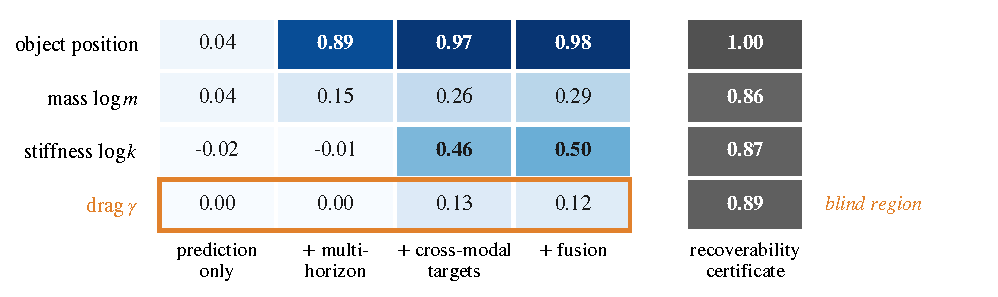
\includegraphics[width=\linewidth]{fig_map.pdf}
\caption{\textbf{The identifiability map.} Linear-probe R\textsuperscript{2}
per physical quantity as the objective is cumulatively enriched (columns;
\pokeworld{}, contact windows), against recoverability certificates (lower
bounds from raw observations; nonlinear probes agree, App.~\ref{app:results}).
Multi-horizon pressure recovers visible state, cross-modal targets recover
contact physics, and one certified-recoverable parameter (boxed) is acquired
by none---the frontier these objectives leave open.}
\label{fig:map}
\end{figure}

This paper charts that map. We build \pokeworld{}, a minimal interactive environment
in which a force-controlled agent pokes objects whose hidden parameters---mass $m$,
drag $\gamma$, contact stiffness $k$---are resampled every episode and rendered
\emph{identically}: nothing about appearance reveals them. The three parameters
deliberately span an observability spectrum ($\gamma$ chiefly visual, $m$
cross-modal, $k$ almost purely tactile), so \emph{which} representation acquires
\emph{which} parameter is diagnostic of the learning dynamics. Every claim passes the
\emph{certificate gate}: a recurrent probe on raw observations must certify
a parameter as recoverable before any statement about a model is made. The
gate separates environment defects from representation defects---and
instrument defects from both---licensing the causal language used
throughout.

On this substrate we train \xjepa{}, a family of action-conditioned latent world
models built on the heuristic-free LeJEPA/LeWM recipe
\citep{balestriero2025lejepa,maes2026lewm}, factorially varying which modalities
enter the \emph{input}, which are prediction \emph{targets}, and the horizon
spectrum of prediction heads. Linear probes on the frozen predictor state, read
against the recoverability certificates, measure what was learned. Four
findings define the map, answering in turn what is recoverable, what the
objective retains, and what stays systematically absent:

\textbf{1. Target pressure is causal and modality-specific
(\S\ref{sec:pressure}).} Contact stiffness enters the latent only when touch is a
prediction \emph{target} (R\textsuperscript{2} $0.40$--$0.57$ across seeds,
regularization strengths, two architectures, and probe families)---not when
touch is merely fused into the input ($-0.02$), nor when an equally sized
proprioception target substitutes for it ($-0.01$). Mass rises monotonically
with cross-modal pressure, and targets \emph{compose} for object localization
($0.58$ vs.\ $0.17$/$0.09$ alone).

\textbf{2. Vision-only latent world models sit in a lazy equilibrium
(\S\ref{sec:lazy}).} With single-step prediction they discard even directly
visible, perfectly predictable object state (position R\textsuperscript{2}
$0.04$)---\emph{visible, predictable, ignorable}. Two independent mechanisms
break the degeneracy---cross-modal targets ($\rightarrow 0.58$) and
multi-horizon action-conditioned heads ($\rightarrow 0.89$)---and they compose
($0.98$); direct long-horizon heads also outpredict autoregressive composition
at matched horizons ($0.10$ vs.\ $0.19$ arena units; static $0.21$).

\textbf{3. The anti-collapse regularizer sets metric precision
(\S\ref{sec:lambda}).} Sweeping the weight of SIGReg (the recipe's sliced
isotropic-Gaussian anti-collapse regularizer) over $60\times$ traces a
monotone dose--response on every physical readout (stiffness $0.12 \rightarrow
0.57$; prediction error halves): distributional regularity trades against the
latent's metric precision, and low-intrinsic-dimension data wants an
order-of-magnitude lighter regularization than image-scale defaults.

\textbf{4. The map has a frontier (\S\ref{sec:frontier}).} Drag $\gamma$ carries a
recoverability certificate of R\textsuperscript{2} $0.89$ yet resists every
prediction-side mechanism we deploy---across linear probes, nonlinear probes, and
a functional test of the model's own glide predictions---plateauing near $0.13$.
A supervised head on the same trunk reaches $0.45$ with prediction
quality unchanged, and a pixel-reconstruction variant is at least as blind:
the failure sits with the deterministic prediction objectives we test, not
with the environment or the probes. An attribute matrix with dose--response
interventions then yields a two-regime picture: fast parameters are acquired
through whatever computation their readout requires; slow parameters only up
to their \emph{linear} observational trace (a bias family swept over three
signal levels tracks its linear certificate while its recurrent certificate
stays near $0.95$); and slow, ratio-type parameters, having no linear trace,
are blind---immune even to a $30\times$ loss reweighting.
Real-world parameters with this signature---viscosity, friction---are what
contact-rich robotics needs; the frontier is a concrete target for the next
generation of objectives.

\textbf{Real-robot validation at scale (\S\ref{sec:real}).} On RH20T
\citep{fang2023rh20t} across two embodiments ($896$ and $4{,}258$
episodes), the map's mechanisms transfer, evaluated on observables with
held-out tasks throughout:
the lazy equilibrium replicates verbatim; cross-modal targets improve dynamics
prediction ($-29\%$ rollout error) and contact anticipation (AUC $0.70 \rightarrow
0.80$); force is retained, and forecast beyond a persistence baseline, only
when touch is both fused \emph{and} forecast. Camera viewpoint acts as
an \emph{observable selector}, a two-view model taking the union. Most
consequentially, a four-arm factorial (inputs $\times$ targets) run
across within-embodiment scaling ($800$--$4{,}258$ episodes, fixed compute,
$+50\%$-compute control) separates sensor observability, input fusion, and
prediction pressure: every arm missing a factor is \emph{flat in
scale}---the camera-only arms never gain force information no view carries,
and the fused-input arm without cross-modal targets discards the force it is
given---while the full objective is near-ceiling from $800$ episodes and
converts additional scale into held-out-task gains. \textbf{Scale cannot
substitute for objective structure}: multi-sensory pressure decides what can
be learned, and only then does data decide how well.

\textbf{Contributions.} (1)~\pokeworld{} and the certificate-gated identifiability
protocol: a reusable methodology turning ``what did the model learn?'' into a
controlled measurement. (2)~The four-factor identifiability map---target
causality, the lazy equilibrium and its escapes, the $\lambda$
dose--response. (3)~The frontier: a certificate-gated attribute-matrix
characterization of what these objectives do not acquire, with
objective-attribution controls. (4)~Real-robot validation across two
embodiments, culminating in a four-arm factorial over scaling curves showing
that objective structure---not data volume---decides what is learned, with
distilled design rules.

% ==========================================================================
\section{Related Work}
\label{sec:related}

\textbf{Latent world models and JEPAs.} Predicting future latent embeddings
rather than observations underlies I-JEPA and V-JEPA
\citep{assran2023ijepa,assran2025vjepa2}, with action-conditioned variants
supporting zero-shot planning \citep{assran2025vjepa2,zhou2024dinowm}. LeJEPA
replaces the stability heuristics of this line (EMA teachers, stop-gradients)
with a single principled regularizer, SIGReg \citep{balestriero2025lejepa},
which LeWorldModel instantiates as a stable end-to-end pixel world model
\citep{maes2026lewm}. We adopt this recipe as our substrate and contribute a
systematic account of what its representations acquire---including a
dose--response analysis that turns LeWM's observation that SIGReg can struggle
on low-complexity environments into an actionable tuning rule. Generative world
models \citep{hafner2023dreamerv3} optimize reconstruction; we study the
latent-predictive family and include a reconstruction-objective control on the
same trunk (\S\ref{sec:frontier}), which reproduces the blind region.

\textbf{Touch and multimodal representation.} Touch supplies physical evidence
vision lacks: Sparsh learns self-supervised tactile representations
\citep{sparsh2024}, TacGen shows contact-dependent properties become decodable
only with a tactile channel \citep{tacgen2026}, TouchWorld builds a generative
visuo-tactile policy stack \citep{touchworld2026}, Kepler-Encoder fuses
vision, proprioception, and force into a static multimodal embedding
\citep{kepler2026}, and HPT scales proprioceptive--visual pretraining across
embodiments \citep{hpt2024}. We study \emph{action-conditioned dynamics}
models and dissect the causal roles of inputs versus prediction targets---a
distinction invisible to static-encoder studies, and one that reshapes how
multimodal world models should be trained. Auxiliary prediction objectives
shaping representations have RL antecedents \citep{jaderberg2017unreal,
gelada2019deepmdp,guo2020pbl}; our contribution is the input-versus-target
dissection under recoverability certificates, not target-driven content per
se. Estimating physical parameters from video and interaction is likewise
established \citep{wu2015galileo,wu2016physics101,xu2019densephysnet}: that
line supplies the recoverability side, where we measure what
prediction-trained latents acquire relative to it.

\textbf{Physical understanding, probing, and identifiability.} Benchmarks probe
pretrained video models for intuitive physics \citep{garrido2025intuitive} and
physical principles \citep{physicsiq2025}; we complement post-hoc evaluation
with a \emph{controlled} methodology whose roots are classical: parameter
identifiability and the role of input excitation are foundational in system
identification \citep{ljung1999system}, and our certificates and behavior-policy
design transpose them to learned latents. From the probing literature we import
its central caution---probe results reflect probe capacity as much as
representation content \citep{hewitt2019control,belinkov2022probing}---which is
why every claim here is triangulated across linear probes, nonlinear probes,
recoverability certificates, and functional prediction tests. The lazy
equilibrium is a world-model instance of shortcut learning
\citep{geirhos2020shortcut}: the objective is satisfiable while ignoring
task-relevant structure. On the theory side, JEPA objectives have
been characterized as low-rank factorization of action-conditioned
co-occurrences \citep{jepatheory2026}, SIGReg as an active-inference free
energy \citep{sigregfe2026}, and data-averaged prediction error as insufficient
to bound planner suboptimality \citep{controltheory2026}; the lazy equilibrium,
the blind region, and the scale-flat degeneracy supply concrete phenomena for
such theories to explain.

% ==========================================================================
\section{\pokeworld{} and the Certificate-Gated Protocol}
\label{sec:setup}

\begin{figure}[t]
\centering
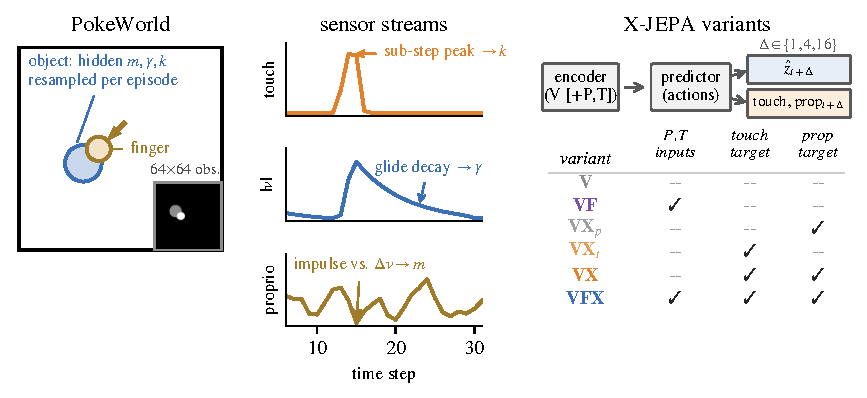
\includegraphics[width=\linewidth]{fig_setup.pdf}
\caption{\textbf{\pokeworld{} and the X-JEPA factorial.} Left: a
force-controlled finger interacts with an object whose mass, drag, and
stiffness are resampled every episode and never visible (inset: the actual
$64{\times}64$ observation). Middle: each sensor stream carries different
physics---sub-step tactile peaks carry stiffness, glide decay carries drag,
impulse--velocity coupling carries mass. Right: the variant family
factorially varies which modalities enter the encoder and which are
forecast; all variants share the trunk and the $\Delta \in \{1,4,16\}$ heads.}
\label{fig:setup}
\end{figure}

\textbf{Environment.} \pokeworld{} (Fig.~\ref{fig:setup}) is a 2D arena in
which a force-controlled
circular finger interacts with an object under semi-implicit Euler dynamics with
Hertzian-style penalty contacts (underdamped, $\zeta{=}0.25$, so that impact
transients survive). Each episode resamples hidden parameters---mass
$m \in [0.5, 3.0]$, drag $\gamma \in [0.5, 4.0]$ (velocity decay rate,
mass-independent by construction), contact stiffness $k \in [500, 6000]$---while
rendering is \emph{identical} across episodes: nothing visual reveals any
parameter (Fig.~\ref{fig:pairs}). Observations comprise vision,
proprioception, and 7-d touch with
\emph{sub-step statistics} (mean, \textbf{peak}, and end-of-step force;
contact duration): quasi-static push force is $k$-independent, so stiffness
lives only in impact transients---the band kHz force--torque sensors occupy
and frame-averaging destroys. Behavior policies mix pursuit,
strike--retreat, and free launches so contacts, impacts, and glides all
occur. Which representation acquires which parameter therefore reads out
the learning dynamics, not the environment (Fig.~\ref{fig:setup}, middle).

\textbf{Recoverability certificates.} Before any model is evaluated, each
parameter must be \emph{certified recoverable} from raw observations
(the full protocol is diagrammed in Fig.~\ref{fig:protocol},
appendix). A certificate is a lower bound: the best R\textsuperscript{2} achieved by any
estimator we construct on raw observation windows---a supervised recurrent
probe for all parameters ($0.86$ for $\log m$, $0.87$ for $\log k$ on contact
windows) and, for drag, a physics-informed estimator reaching $0.89$ where
the recurrent probe reaches $0.70$. Certificates let a null \emph{model}
result be attributed to the objective rather than the environment or the
instrument; the estimator hierarchy is itself informative (linear probes
cannot express the ratio $m = F/a$; windowed MLPs cannot express temporally
gated programs; the recurrent probe expresses both, App.~\ref{app:env}). On
the model side we report linear (ridge) and nonlinear (early-stopped MLP)
probes on the frozen predictor state, plus \emph{functional} tests of the
model's own predictions (\S\ref{sec:frontier}). Throughout, we separate
\emph{recoverable} from observations (certificates), \emph{decodable} from
the latent (probes), and \emph{functionally used} by predictions (glide
tests)---never classical structural identifiability
\citep{ljung1999system}: every statement is operational, under the tested
models, coordinates, horizons, and objectives.

\textbf{\xjepa{} family.} All models share the stable LeJEPA/LeWM substrate:
per-frame encoders, a causal transformer predictor conditioned on actions,
prediction heads at horizons $\Delta \in \{1,4,16\}$, and the SIGReg
anti-collapse objective (weight $\lambda$; architecture in
App.~\ref{app:training}). Variants
factorially vary \emph{inputs} (vision-only vs.\ all modalities) and
\emph{targets} (latent embeddings only; adding touch and/or proprioception
forecasting), as tabulated in Fig.~\ref{fig:setup} (right). Models are
${\sim}5$M parameters and train
in under an hour on a single laptop GPU---the entire study, including all real-robot
experiments, was conducted on one RTX~4060.

\textbf{Measurement.} We probe the frozen predictor state with ridge regression
for hidden parameters (on contact windows, where the certificates are established),
object position and velocity, open-loop rollout and direct-$\Delta$
prediction against a static baseline, and, on real data,
force readout, contact-onset anticipation (AUC), and held-out-task splits.
All probe evaluations are episode-split: probe-fit and probe-test windows
come from disjoint episode sets, and hidden parameters are resampled per
episode.

% ==========================================================================
\section{The Identifiability Map}
\label{sec:map}

\subsection{Targets, not inputs, decide content}
\label{sec:pressure}

Figure~\ref{fig:targets} shows the central factorial at $\lambda{=}0.02$
(two seeds; full table in Table~\ref{tab:targets}, appendix). Three
comparisons carry the causal weight:

\begin{figure}[t]
\centering
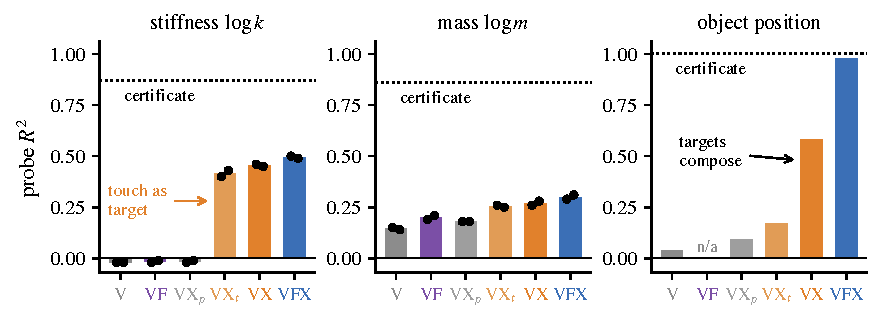
\includegraphics[width=0.86\linewidth]{fig_targets.pdf}
\caption{\textbf{Targets, not inputs, decide hidden-parameter content.} Probe
R\textsuperscript{2} by variant (gray: no touch target; orange: touch target,
vision-only input; blue: full). Stiffness appears only under touch-as-target;
position emerges from target \emph{composition}. Dotted: certificates.}
\label{fig:targets}
\end{figure}

\emph{(i) Touch as input does nothing for stiffness; touch as target does
everything.} VF fuses the full tactile stream into the encoder yet leaves $k$
at chance; VX$_t$ sees \emph{no} touch at input yet reaches $0.40$--$0.43$ by
being asked to \emph{forecast} touch: forecasting contact force under known
actions requires the latent to carry stiffness---so it does.

\emph{(ii) The effect is modality-specific, not generic auxiliary pressure.}
VX$_p$ adds an equally sized proprioception-forecasting target and moves $k$
not at all ($-0.01$): what matters is not extra work, but that the extra
work's answer depends on the parameter. Early-stopped MLP probes reproduce
every cell ($0.40/0.44/0.51$ for VX$_t$/VX/VFX vs.\ $\le 0.00$ for V/VX$_p$;
App.~\ref{app:results}): the ordering is invariant to probe capacity.

\emph{(iii) Targets compose.} Neither single target localizes the object
(position $0.17$ and $0.09$), but together they reach $0.58$: the
proprioception target pins the finger, the touch target pins the object
\emph{relative to} the finger, and the composition pins the object. Adding
fusion (VFX) completes the picture ($0.98$ position, best $m$, $k$). The
ordering reappears on real data (\S\ref{sec:real}) and under a token-based
encoder (dense aligned prediction lifts stiffness to $0.62$): a property of
the objective, not of one architecture. In precise form: inputs bound what can be known; prediction targets decide
what is retained---for hidden parameters, fusion without forecasting
contributes nothing.

\subsection{The lazy equilibrium and its two escapes}
\label{sec:lazy}

Under single-step prediction, the vision-only latent barely contains the
object: position R\textsuperscript{2} $0.04$, despite the object being large,
visible, and trivially predictable. The equilibrium is self-consistent (a
static object contributes almost no prediction loss, so the encoder drops it,
so the jointly learned targets never demand it), and the anti-collapse
regularizer cannot prevent it: it constrains the \emph{distribution} of
embeddings, not their \emph{content}. Two independent interventions break
it: cross-modal targets restore position to $0.58$
(Table~\ref{tab:targets}); multi-horizon action-conditioned heads
($\Delta \in \{1,4,16\}$) restore it to $0.89$ with no additional
modality---over 16 steps the object's future position is a large,
action-dependent effect the objective can no longer ignore---and the two
compose to $0.98$. The heads bring a second benefit: at matched horizon, the
\emph{direct} $\Delta{=}16$ head decodes to $0.10$ arena-unit error where
autoregressive composition reaches $0.19$ (static $0.21$)---long-horizon
prediction is best asked for directly, not assembled from rolled short steps.
The equilibrium is a property of the tested class---single-step
global-embedding prediction with jointly learned targets: dense token
prediction restores position by construction (our token variant: $0.98$),
and masked architectures with frozen targets report positional competence
\citep{garrido2025intuitive}---the degeneracy names the failure mode those
designs avoid.

\subsection{The regularizer sets metric precision}
\label{sec:lambda}

Figure~\ref{fig:lambda} (appendix) sweeps $\lambda$ over $60\times$ (full
table in App.~\ref{app:results}). All probes trace the same monotone curve:
the isotropic-Gaussian pressure that guarantees non-collapse also spreads a
low-dimensional physical manifold across the full latent, and the spreading
acts as metric noise on fine-grained readouts. Training remains stable across
the entire range---the practical failure mode on low-intrinsic-dimension data
is over-regularization, not collapse, and the fix is a one-knob adjustment.
This turns a known qualitative concern \citep{maes2026lewm} into a
quantitative tuning rule, and doubles open-loop prediction quality for free.

\subsection{Information, computation, and data coverage}
\label{sec:threefactors}

\emph{Information bandwidth} is set at the sensor: with frame-averaged touch,
stiffness is unrecoverable even from raw observations---averaging destroys
the impact transients---while sub-step tactile statistics restore the
certificate to $0.87$.
\emph{Computation} converts derivatives into measurements: a frozen
self-supervised flow estimator as an input channel raises velocity readout
from $0.79$ to $0.88$ on the same data and objective. \emph{Data coverage}
allocates the gradient mass acquisition runs on: the identical VFX objective
trained on contact-poor data collapses stiffness from $0.50$ to $0.05$ and
mass to $0.11$---the objective can only identify parameters in regimes the
data visits. With target pressure (\S\ref{sec:pressure}), these complete the
map's four levers, each isolated by its own intervention.

\subsection{The frontier: a certificate-gated blind region}
\label{sec:frontier}

Drag $\gamma$ is where the map ends---and the certificate makes the ending
informative: a physics-informed estimator certifies $\gamma$ recoverable at
$0.89$ from state trajectories ($0.43$ from pixel-derived observables,
App.~\ref{app:results}), a self-supervised flow sensor certifies the
derivative information reaches the input, and multi-horizon heads certify
long-horizon pressure. Yet across six families of prediction-side
mechanisms (App.~\ref{app:results}), $\gamma$ plateaus near $0.13$ under
both probe families, and a
functional test shows the model's own glide predictions are beaten by an
estimator that simply assumes the population-median $\gamma$.

\emph{The failure is the objective's---and not one objective's.} A
supervised system-identification head (same trunk, data, optimizer)
lifts $\gamma$ from $0.12$ to $0.45$ (mass and stiffness likewise,
Table~\ref{tab:matrix}) with 16-step prediction unchanged: the
substrate carries the parameter the moment the objective asks. And
swapping latent targets for pixel-reconstruction targets (a deconv
decoder on the same trunk---the core signal of generative world models)
leaves $\gamma$ at least as blind ($0.03$--$0.08$ under both
probe families) while \emph{replicating} the touch-target mechanism
(stiffness $0.61$): blind region and target causality are shared by both
\emph{deterministic point-prediction} families we test, latent-target and
pixel-target alike. The gap that remains between supervision ($0.45$) and
certificate ($0.89$) marks what the current trunk and history length leave
unrecovered even when the objective asks.

Where exactly does acquisition stop? Four candidate attributes distinguish
$\gamma$ from the learned parameters: \emph{slow} (the parameter's per-step
effect on predicted observations lies below the per-channel noise
floor---here, sub-pixel displacement and velocity increments below the
readout residual; a \emph{fast} parameter exceeds it within single events),
\emph{ratio-type} (its readout from the
model's observation coordinates requires divisions rather than linear
functionals---an attribute of the parameter--sensor pair, not of the
parameter alone), temporally \emph{gated} (informative only on glide
segments), and \emph{low variance-share}. An attribute matrix plus two
dose--response interventions separates all four. Each cell carries two
certificates where they differ---a linear probe on raw windows (the
parameter's linearly-accumulable trace) and a recurrent probe (its full
window-recoverable content); both are empirical lower bounds, so every ratio
compares the model to the best estimator we constructed (quoted fractions
are therefore upper bounds on the truly acquired share).
Table~\ref{tab:matrix} carries the result. Stiffness, the fast parameter, is
acquired at $0.6$--$0.7$ of its certificate although no linear functional
reads it: when the parameter is fast, the objective installs whatever
computation its readout needs. The additive bias family, swept over three
signal levels at fixed structure, decides what slowness does: its recurrent
certificate stays near $0.95$ at every level, yet the model tracks the
\emph{linear} certificate instead---a slow parameter is acquired only
through its linear trace. The two slow$\times$ratio parameters, which have
no linear trace, are not acquired at all. And variance-share is a throttle,
not a key:

\begin{table}[t]
\caption{\textbf{The attribute matrix: slow parameters are acquired only
through their linear trace.} Linear and recurrent recoverability
certificates (both empirical lower bounds) against the trained model's
readout; the bias family sweeps signal level at fixed additive structure.
Controls on the same trunk: a supervised head reaches
$m/\gamma/k = 0.72/0.45/0.91$; a pixel-reconstruction objective is at least
as blind on $\gamma$ ($\le 0.08$). Full version with nonlinear probes in
App.~\ref{app:results}.}
\label{tab:matrix}
\begin{center}
\small
\begin{tabular}{llccc}
\toprule
\rowcolor{tabhead} Cell & Parameter & Linear cert.\ & Recurrent cert.\ & Model \\
\midrule
fast$\times$ratio & stiffness $k$ & ${\approx}0$ & $0.87$ & $0.50$--$0.62$ \\
slow$\times$linear & bias $b \in \pm0.5$ & $0.13$ & $0.92$ & $0.13$ \\
 & bias $b \in \pm1.5$ & $0.51$ & $0.96$ & $0.39$ \\
 & bias $b \in \pm2.5$ & $0.65$ & $0.96$ & $0.65$ \\
slow$\times$ratio, gated & drag $\gamma$ & ${\approx}0$ & $0.89$ & $0.13$ \\
slow$\times$ratio, ungated & gain $g$ & $-0.01$ & $0.69$ & $-0.01$ \\
\bottomrule
\end{tabular}
\end{center}
\end{table}
a $30\times$ reallocation toward glide raises $\gamma$'s decodability only
$0.08 \rightarrow 0.27$ while its functional test \emph{worsens}, and
starving the contact-frame touch loss drives stiffness to zero,
parameter-specifically, with data and certificates unchanged
(App.~\ref{app:results}). This is the \emph{blind-region hypothesis}, an
empirical hypothesis about deterministic prediction objectives under these
observation coordinates: fast parameters are acquired as needed; slow
parameters only through their linear trace; slow, ratio-type parameters not
at all. (The certificate gate polices the matrix itself---it rejected three
entangled constructions and forced the two-certificate protocol,
App.~\ref{app:results}.)

The hypothesis makes a falsifiable coordinate-level prediction: attributes
belong to the parameter--sensor pair, so a coordinate in which drag's trace
becomes \emph{linear} should unblind it. A log-speed input channel does
exactly that ($\Delta \log |v| = -\gamma\,\Delta t$ on glide): $\gamma$'s
linear certificate rises from ${\approx}0$ to $0.52$ and the readout
follows to $0.33$---$0.64$ of it, the fraction at which every
linearly-traced parameter is acquired (App.~\ref{app:results}).
Functional use in position
forecasts, which still requires exponentiating the trace, does not follow.
Mass calibrates a fifth lever, target \emph{precision}: nominally
fast$\times$ratio, it reads at $0.43$ of its pixel certificate where
stiffness reads at $0.64$--$0.79$---its trace routes through the
SIGReg-regularized latent target (the $\lambda$ dose--response,
\S\ref{sec:lambda}, is its throttle), stiffness's through raw-valued touch
heads.

A mechanism consistent with every cell is \emph{conditional-mean collapse}:
under squared-error point prediction, whatever a short history does not pin
down is optimally answered by predicting under the population mean of the
parameter, so nothing pressures an episode-specific belief. The matrix reads
naturally in these terms. Fast parameters sharpen the within-window
posterior enough that the optimal prediction needs them. Additive parameters
leak a linear trace into short-horizon states, and the model carries exactly
that trace---it tracks its \emph{linear} certificate across the bias sweep,
never its recurrent one. Slow$\times$ratio parameters, whose effect on the
loss within any prediction horizon stays below the noise floor, are answered
by the prior mean---which also explains why a $30\times$ loss reweighting
raises decodability without creating functional use. A heteroscedastic
Gaussian-NLL variant, which reweights gradients but leaves the mean-optimum
unchanged, moves nothing ($\gamma$ $0.10$ vs.\ $0.12$)---as the mechanism
requires; objectives whose optimum is not a conditional mean (episode-level
latent variables, belief states) remain the discriminating test.

Beyond the frontier, the same lens applies to viscosity, damping, and
friction---with the caveat the definition already carries: the attributes
belong to the parameter--sensor pair. Whether friction is fast or slow
depends on the sensing (stick--slip transients are fast; smooth sliding is
not), and charting exactly that is what the map and its certificates are
for.

\subsection{Control utility tracks state content}
\label{sec:planning}

The map's content transfers to closed-loop control, and control decomposes
along the map's rows: model-predictive control on the frozen latents
(\emph{same planner, budget, and environment} for every representation;
planner and episode in App.~\ref{app:planning}, Fig.~\ref{fig:plan}) reaches
the goal region in $20\%$ of episodes for the object-blind vision-only
latent, $38$--$44\%$ when either target composition restores object state
(VX$_t$/VX$_p$), and $\mathbf{57\%}$ for the full model (random: $1\%$;
distance metric in App.~\ref{app:planning}). Matched state content
yields matched control whether or not the
latent carries stiffness: the position-goal task discriminates state
acquisition only, and force-limited manipulation is the natural next
benchmark.

% ==========================================================================
\section{Real-Robot Data: the Mechanisms Transfer}
\label{sec:real}

Real scenes carry no ground-truth mass or stiffness, so this section tests
whether the map's \emph{mechanisms}---lazy equilibrium, target pressure,
fusion, and their scaling behavior---govern real multimodal streams. We port
the recipe unchanged to RH20T \citep{fang2023rh20t}: a KUKA and a Flexiv
arm ($896$ and $4{,}258$ episodes; corpus details App.~\ref{app:real}),
$10$\,Hz, single $96{\times}96$ camera unless stated; episode-level
splits, every headline metric also reported on \emph{entirely held-out
tasks}. Metrics are observation-space:
force and end-effector position readout from the latent, open-loop and
direct 16-step prediction vs.\ a static baseline, and contact-onset
anticipation (AUC; definition in App.~\ref{app:real}). By the map's own
bandwidth lever, $10$\,Hz force sampling removes stiffness-type transients:
the contact-parameter frontier is out of reach on this corpus by
construction, and what transfers is the mechanism set.

\begin{figure}[t]
\centering
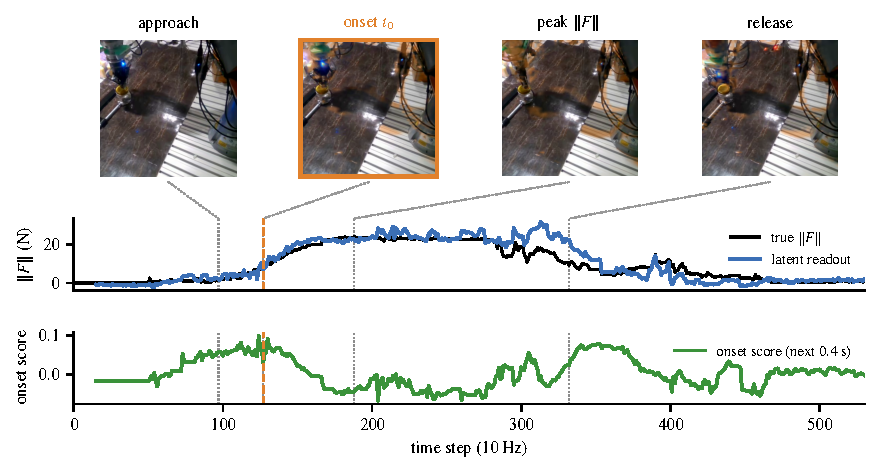
\includegraphics[width=0.81\linewidth]{fig_qual.pdf}\\[4pt]
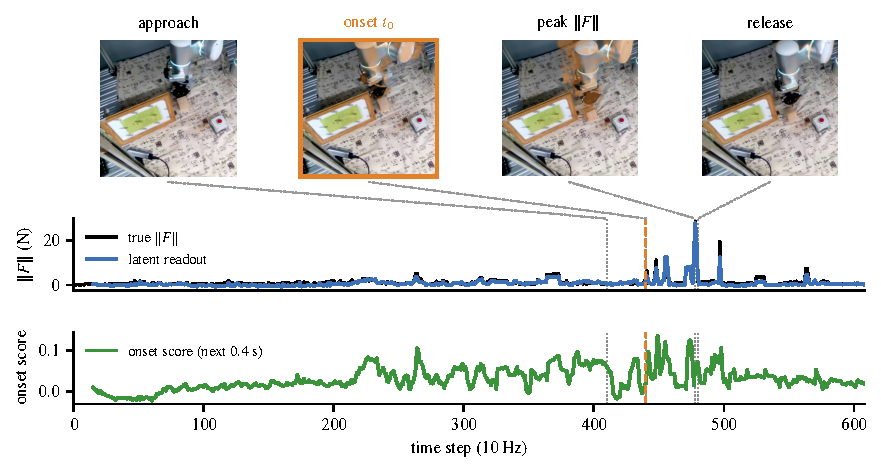
\includegraphics[width=0.81\linewidth]{fig_qual_b.pdf}
\caption{\textbf{The latent reads contact physics on held-out real episodes,
on both embodiments.} Top block: KUKA (53\,s); bottom block: Flexiv (61\,s).
Each block shows camera frames at four interaction phases (native-resolution
color, cropped to the manipulation zone and brightened for display---the
model consumes $96{\times}96$ grayscale; orange overlay marks change since
the previous panel; dotted connectors mark each frame's time), force
magnitude read \emph{from the frozen latent} (blue) against
the wrist sensor (black), and the trunk's onset score, which rises
\emph{ahead of} contact ($t_0$, dashed; dotted: frame times)---anticipation,
not detection. KUKA traces a full press-and-release arc; Flexiv resolves a
train of sharp impulses peak by peak.}
\label{fig:qual}
\end{figure}

\textbf{The lazy equilibrium replicates; targets improve dynamics.}
Vision-only V loses end-effector state (position $0.76$ IID, $0.48$ OOD) and
predicts \emph{worse than static} ($8.2$ vs.\ $3.8$\,cm). Cross-modal
targets (VX, VX$_t$) cut rollout error up to $29\%$ and lift anticipation
AUC $0.70 \rightarrow 0.80$---the toy's target-pressure mechanism on real
streams.

\textbf{Fusion under target pressure delivers force; viewpoint selects
observables.} With force--torque fused \emph{and} forecast as a target, VFX
retains force ($0.87$; OOD $0.56$), predicts 16 steps at $1.5$\,cm
($2.5\times$ better than static), and anticipates contact at AUC
$0.86$.
For camera-only latents the camera decides \emph{what} can be known: a
far view carries pose but not contact, a close-up the reverse, and a
two-view model takes the union (per-viewpoint numbers in
App.~\ref{app:real}). Viewpoint is an \emph{observable selector},
multi-view its union operator.

\begin{figure}[t]
\centering
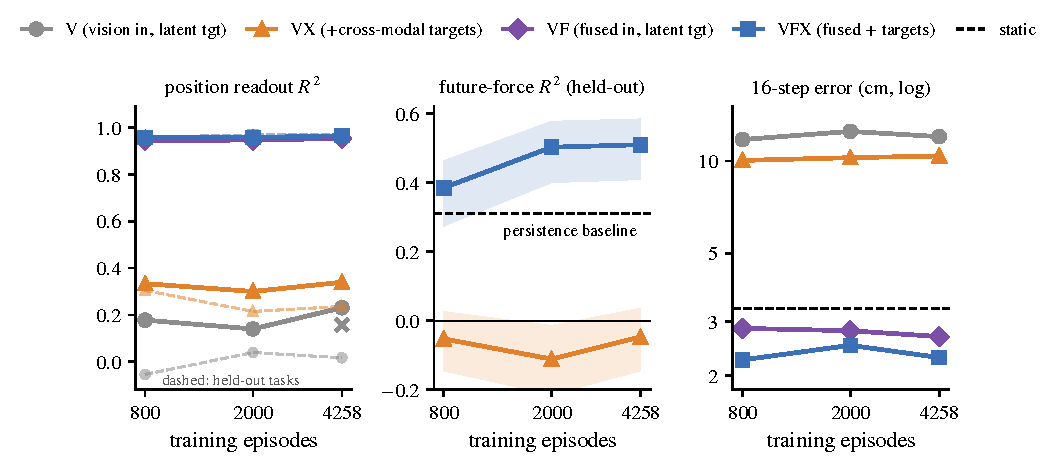
\includegraphics[width=0.79\linewidth]{fig_scissors.pdf}
\caption{\textbf{The four-arm factorial across scale.} Flexiv,
within-embodiment (identical robot, tasks, viewpoint, protocol; fixed
compute; $\times$: $+50\%$-compute control). Left: position readout---the
fused-input arms sit at the passthrough bound regardless of targets (dashed:
held-out tasks). Center: future-force forecasting on held-out tasks---the
passthrough-immune force metric: VFX beats persistence at every scale and
improves with data; VX never matches persistence. Right: direct 16-step
error---the factors compose; V stays ${\sim}4\times$ worse than static at
every scale.}
\label{fig:scissors}
\end{figure}

\textbf{The factorial at scale: scale cannot buy back what the objective
refuses.} Readout metrics on fused-input models can be input-driven, so we
bound the trivial component first: an \emph{untrained} copy of the fused
architecture, probed identically, already reads force at $0.94$ and position
at $0.97$---random projections pass inputs through. Read against this bound,
the $2{\times}2$ factorial (inputs $\times$ targets), run across
within-embodiment scaling ($800$--$4{,}258$ episodes at fixed compute, with
a $+50\%$-compute control), assigns every metric its cause
(Fig.~\ref{fig:scissors}; App.~\ref{app:results}). Position readout is
passthrough: the fused arms sit at the bound at every scale, and the
vision-only model sits at its \emph{own} random-feature bound across the
whole range---more compute does not change this.
Force is where the factorial bites, and \emph{forecasting} is its honest
metric: current-force readout is passthrough-bounded, so the center panel
asks the passthrough-immune question instead---predict force $0.4$\,s
ahead. VFX
beats the persistence baseline at every scale and its forecast
\emph{improves} with data ($0.39 \rightarrow 0.51$ held-out)---the one
metric where scale clearly pays (episode-bootstrap CIs,
App.~\ref{app:results}); VX stays below persistence at every scale, because
no amount of data supplies information the camera does not carry. The retention view (Fig.~\ref{fig:forceread}, appendix) confirms the
factorial: VF, which \emph{receives} force as an input, lands far below
the untrained bound ($0.15$ vs.\ $0.91$)---training compresses away a
sensed modality nothing pressures it to keep. The same signature runs through every learning metric: direct
16-step error improves monotonically as factors add ($12.0 \rightarrow
2.3$\,cm; static $3.3$), and camera-only anticipation is
learned (AUC $0.62 \rightarrow 0.77$) while fused-model anticipation sits at
its random-feature bound. Cross-robot differences that look like scale effects are the viewpoint
lever again (App.~\ref{app:real}). \textbf{Objective structure decides
what can be learned; data decides only how well.}

\textbf{One model, two robots.} A single \emph{configuration-blind} VFX
trained jointly on both corpora (no robot identifier) matches both
specialists on position and anticipation and lifts the data-poor KUKA side's
force retention from $0.56$ to $\mathbf{0.89}$ on held-out tasks: pooled
cross-embodiment experience supplies the task coverage that stabilizes
retention. Another
robot's experience is not interference but coverage.

% ==========================================================================
\section{Design Rules}
\label{sec:discussion}

The map compresses into rules, each backed by a controlled comparison:

\begin{enumerate}[itemsep=1pt,topsep=3pt,parsep=0pt]
\item \textbf{Every modality a prediction target}---un-forecast fusion is
discarded; forecast touch to know stiffness.
\item \textbf{Sense at the physics' bandwidth}---sub-step tactile
statistics, motion channels, derivative estimators.
\item \textbf{Ask for the future at multiple horizons, directly}---breaks
the lazy equilibrium; beats autoregressive composition.
\item \textbf{Tune anti-collapse to the data's intrinsic dimension}---an
order of magnitude lighter on physical data.
\item \textbf{Structure first, scale second}---arms missing information or
pressure stay flat across a $5\times$ range.
\end{enumerate}

\section{Limitations}
\label{sec:limitations}

Both tested objectives are deterministic point predictions on one trunk.
Objectives whose optimum is not a conditional mean, such as
episode-level latent variables or belief states, are the discriminating
test for the mechanism we propose, and they lie outside the family this
study scopes; our Gaussian-NLL control is the closest variant we run,
and it moves $\gamma$ not at all. Blind-region statements are scoped
accordingly. Second, the real-robot sections validate the map's
\emph{mechanisms} on observables rather than parameter identifiability
itself, since RH20T has no ground-truth object parameters; the direct
test is a corpus of objects with known, varied physical parameters.
Third, models are ${\sim}5$M parameters on one GPU: what transfers is
the protocol, not the ceiling.

\section{Conclusion}
\label{sec:conclusion}

We asked which physical quantities a prediction-trained latent contains.
Certificates separate what the environment affords from what the
objective acquires, and under that separation the answer is narrower
than the premise we started from. A latent carries the parameters its
prediction targets require of it, while a modality that is fused but
never forecast contributes nothing. Additional data changes this in no
arm that lacks either the information or the prediction pressure. One
class of certified-recoverable parameters is acquired by none of the
objectives we test, and naming that class precisely is what the
environment and its certificates are for.

\subsubsection*{Reproducibility statement}
The environment, protocol, and all evaluation code run on one consumer GPU;
exact configurations are in the appendix, and code will be released.

\label{endofmain}
\bibliography{refs_generated,preprint}
\bibliographystyle{preprint}

\appendix
\raggedbottom
\section{Environment and Protocol Details}
\label{app:env}

\begin{figure}[H]
\centering
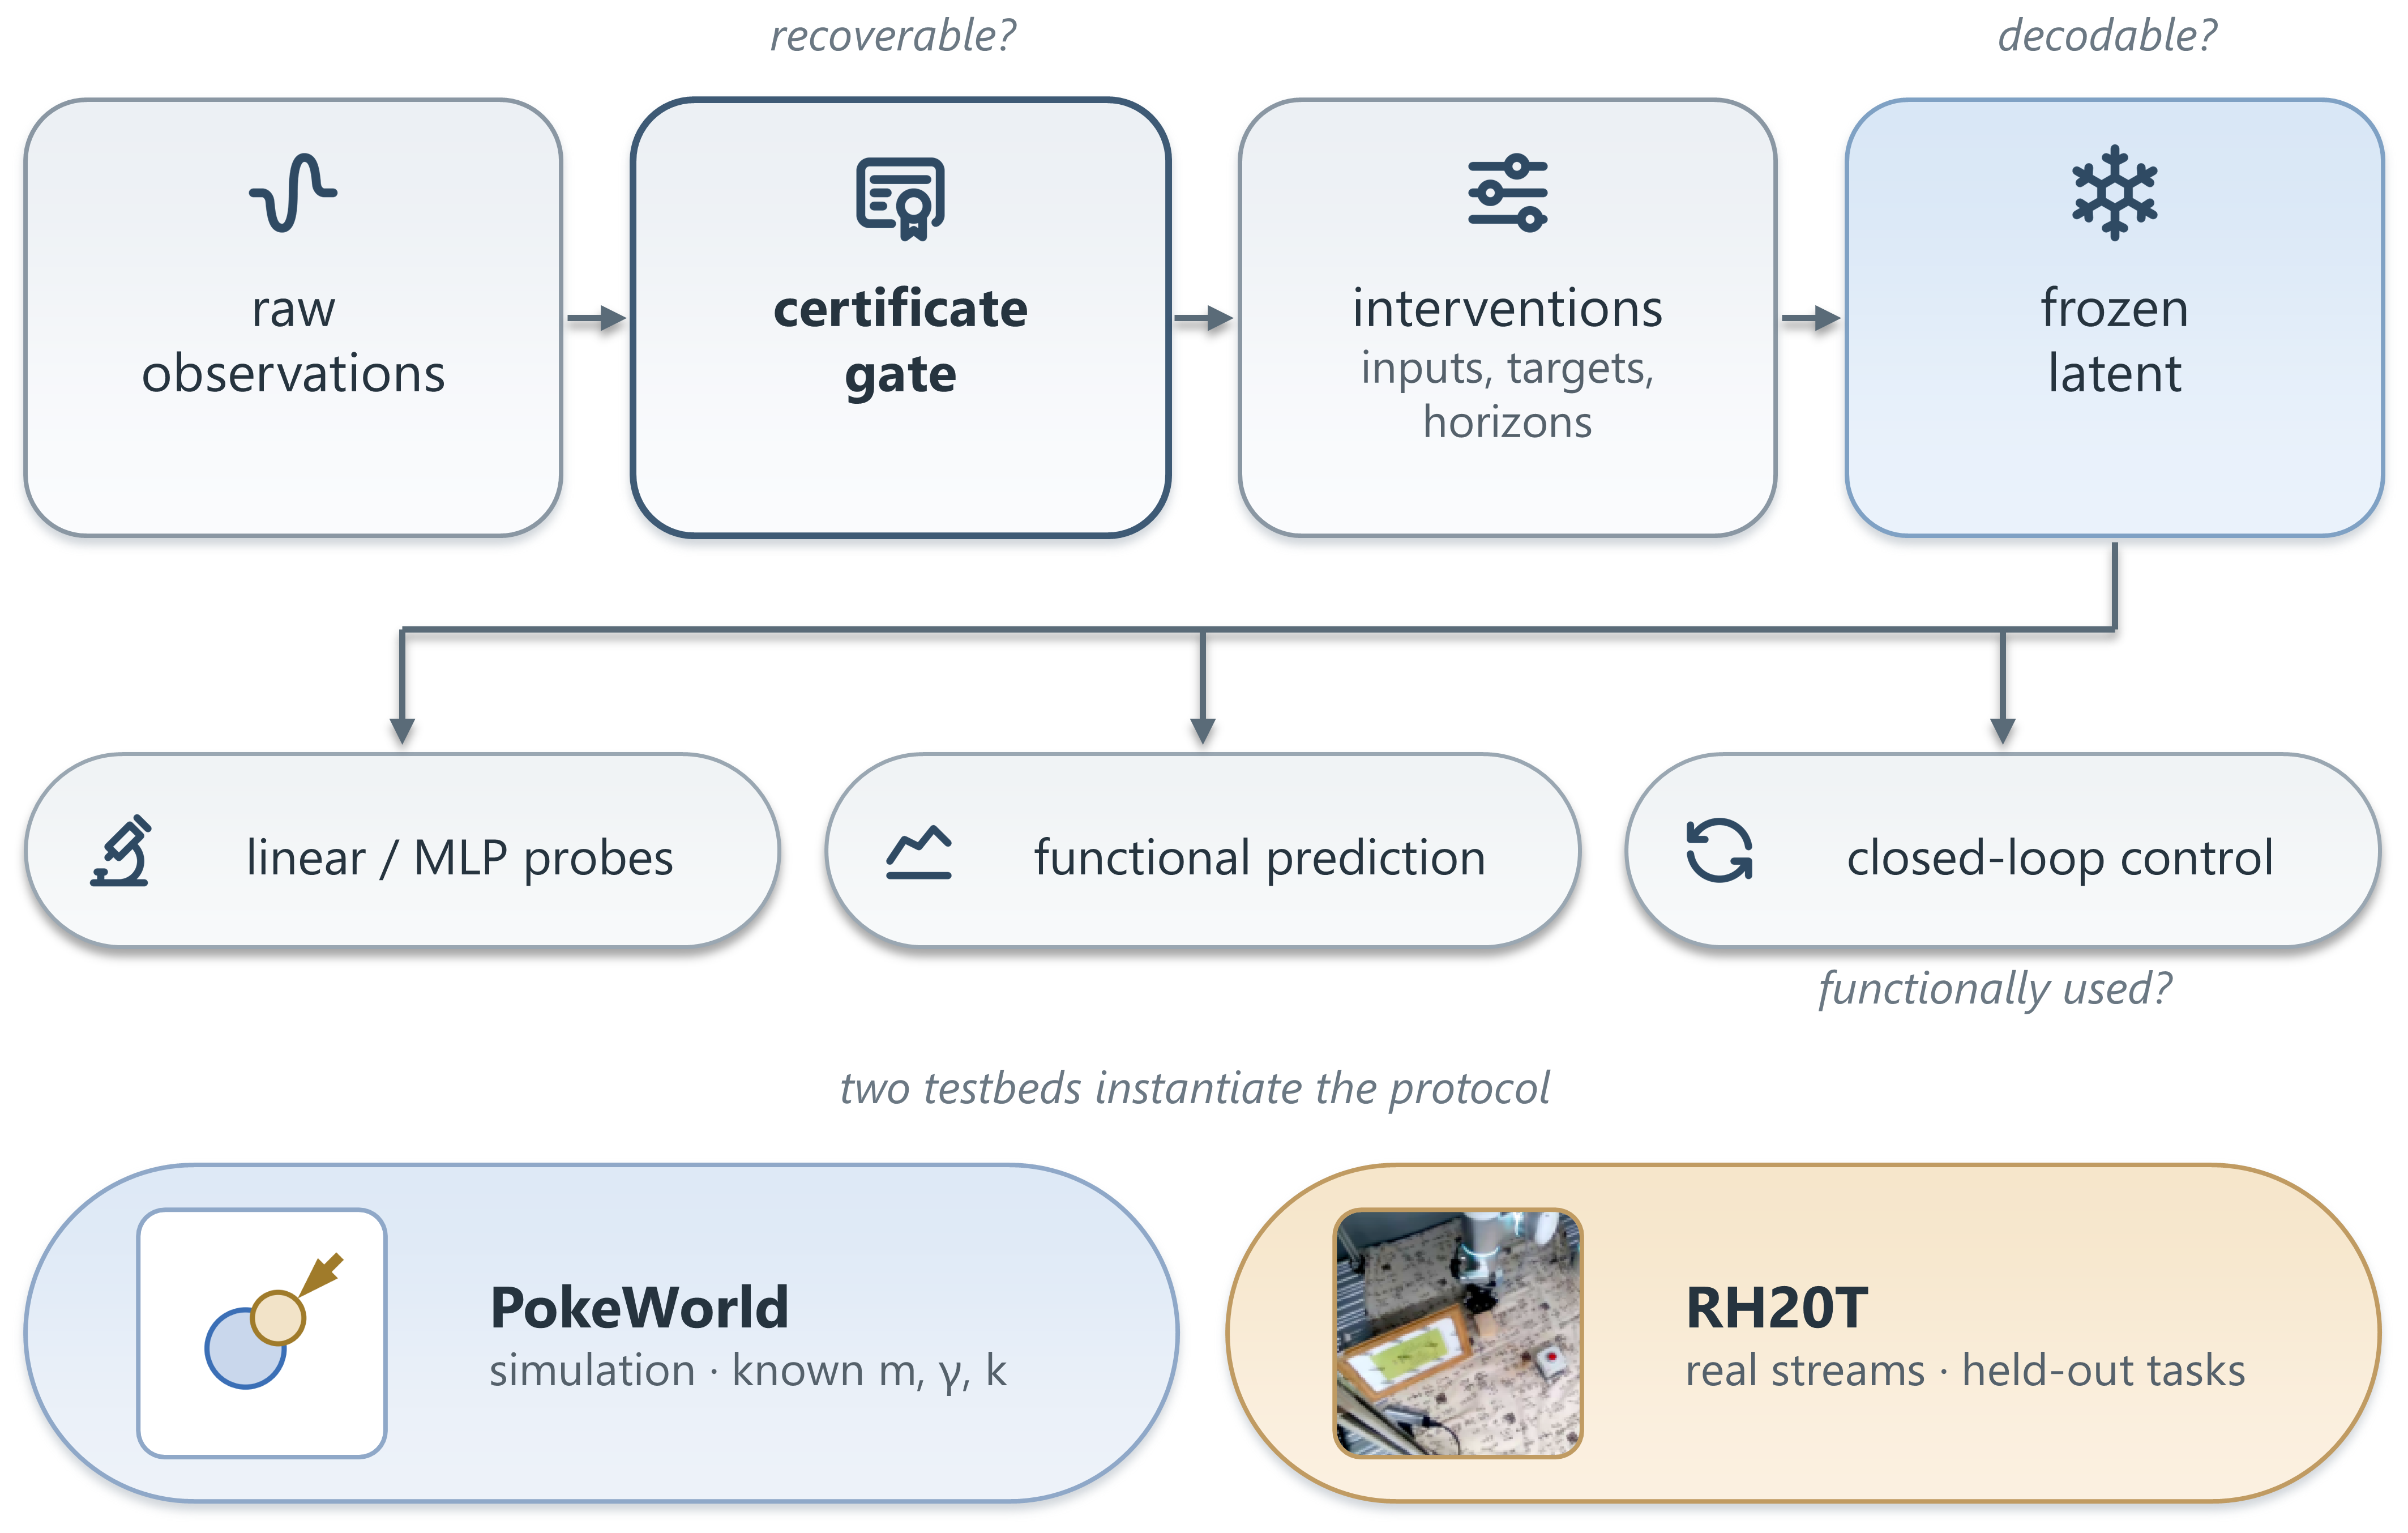
\includegraphics[width=\linewidth]{fig_protocol.png}
\caption{\textbf{The certificate-gated protocol.} Every claim in the
paper follows this path. Raw observations must first certify a
parameter as recoverable (\emph{recoverable?}); input, target, and
horizon interventions then train variants on identical data; and the
frozen latent is read by probes (\emph{decodable?}) and by functional
prediction and closed-loop control (\emph{functionally used?}). Two
testbeds instantiate it: \pokeworld{}, where the hidden parameters are
known by construction, and RH20T, where only observables and held-out
tasks are available.}
\label{fig:protocol}
\end{figure}

\textbf{Dynamics.} Bodies follow semi-implicit Euler integration at
$\mathrm{d}t{=}0.05$ with 20 substeps. The finger (mass $1$, radius $0.06$) is
driven by a commanded force $F_{\max} a_t$, $a_t \in [-1,1]^2$; the object
(radius $0.09$) experiences drag force $-\gamma m v$ (so the velocity decay
rate $\gamma$ is mass-independent by construction), and finger--object contact
follows a Hertzian penalty law $F_c = k\,d^{3/2}$ with normal damping at
$\zeta{=}0.25$ of critical, where $d$ is the overlap. Underdamping matters:
near-critical damping makes impact peaks damping-dominated and suppresses the
stiffness signature that the tactile channel must carry. Parameters are sampled
log-uniformly ($m \in [0.5,3]$, $k \in [500,6000]$) or uniformly
($\gamma \in [0.5,4]$) per episode.

\begin{figure}[H]
\centering
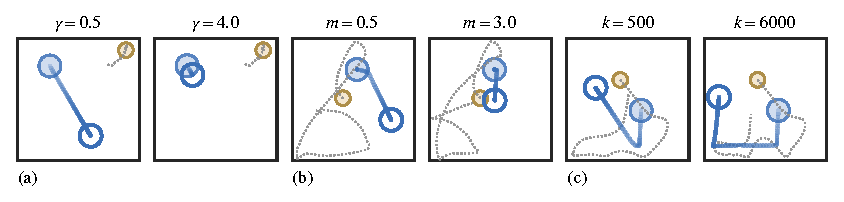
\includegraphics[width=\linewidth]{fig_pairs.pdf}
\caption{\textbf{Nothing in the rendering reveals a hidden parameter.}
Three matched pairs of \pokeworld{} episodes. Within a pair the episodes
start from an \emph{identical} frame and are driven by an \emph{identical}
action sequence; only one hidden parameter differs. Filled circles mark the
start (object blue, finger gold), the hollow circle the object's final
position, the blue path its trajectory (light to dark with time), and the
dotted path the finger. (a) drag: the low-drag object glides across the
arena while the high-drag one stops almost immediately. (b) mass: the same
strike sends the light object far and barely moves the heavy one.
(c) stiffness: the impact transient differs, and with it the post-contact
trajectory. Appearance is identical at every step---only the physics is
not.}
\label{fig:pairs}
\end{figure}

\textbf{Sensors.} Vision renders anti-aliased $64{\times}64$ grayscale; the
model input adds a temporal-difference channel. Proprioception is finger
position and velocity (4-d). Touch reports per-control-step sub-step
statistics of the reaction force on the finger: mean force (2-d), peak
magnitude, end-of-step force (2-d), contact duration fraction, and a contact
flag (7-d total). Sensor noise $\sigma{=}0.02$ is added to force channels.

\textbf{Behavior policy.} Episodes (64 steps) mix three modes with random
switching---pursuit (sustained pushes), strike--retreat cycles (clean impacts
followed by free glides), and Ornstein--Uhlenbeck drift---plus a fraction of
episodes in which the object is launched with random velocity, so that
contacts, impacts, and glides all appear in the marginal data distribution.

\textbf{The oracle estimator.} The oracle is a 2-layer GRU (width 96) over
16-step windows of raw observations, trained directly on the parameter
labels. Gates require contact-window R\textsuperscript{2} of at least
$0.4/0.4/0.25$ for $m/\gamma/k$ before any model result is interpreted.

\textbf{Instrument hierarchy.} Instrument choice is itself part of the
protocol. A \emph{linear} probe on raw windows cannot express the ratio
$m = F/a$ and scores near zero on all three parameters. A windowed
\emph{MLP} recovers mass ($0.45$) but scores $0.0$ on drag, even though a
hand-written estimator (the median log velocity-ratio over glide frames)
reaches $0.89$: drag is a \emph{temporally gated} program that flat
architectures do not express. The recurrent oracle expresses both program
classes and sets the certificates used throughout ($0.86/0.70/0.87$).
Certificate estimators read trajectories of finger state (proprioception),
touch, actions, and object state; object state is privileged relative to
the pixel channel, and pixel-derived counterparts are reported in
App.~\ref{app:results}. The same discipline applies on the model side: reported probes are ridge
regressions, so every claimed acquisition is \emph{linearly} available in
the latent, and the functional glide test (App.~\ref{app:results})
separately checks whether the model's own predictions \emph{use} a
parameter.

\section{Training Details}
\label{app:training}

\textbf{Architecture.} All models share per-frame encoders---a 4-stage CNN
(channels $32/64/128/256$, stride 2) over the frame and temporal-difference
channels, with small MLPs for proprioception and touch---fused and projected
through a linear layer with \emph{BatchNorm}. There is deliberately no
trailing LayerNorm: a final LayerNorm constrains embeddings to a shell and
blocks the isotropic-Gaussian target of SIGReg, reproducing the observation
of \citet{maes2026lewm}. The predictor is a 4-layer causal transformer
(width 192, 8 heads, dropout 0.1) with zero-initialized AdaLN action
conditioning. Prediction heads at $\Delta \in \{1,4,16\}$ condition on the
flattened intervening action window, and cross-modal forecasting heads
(touch, proprioception) sit on the trunk where the variant specifies. The
latent dimension is 128.

\textbf{Optimization.} AdamW at learning rate $3{\times}10^{-4}$ with cosine
decay and 500-step warmup, weight decay $0.05$, batches of 96--128 windows
of 24 frames, 20k steps, bf16 autocast. SIGReg uses 1024 random directions
with 17 integration knots, resampled every step.

\textbf{Token-level SIGReg.} For token-based variants, SIGReg is evaluated
on 4096 subsampled token rows with 256 directions per step. Per-step
resampling preserves coverage while cutting the regularizer's activation
memory by two orders of magnitude---the change that makes token-level SIGReg
practical at all.

\textbf{Control variants.} The reconstruction control replaces the latent
targets with a shared deconvolutional decoder (four stride-2 upconvolutions
from a $4{\times}4$ map, channels $256/128/64/32$) fed by per-horizon
adapters (action-conditioned for $\Delta > 1$), decoding 8 uniformly
subsampled positions per window and horizon; the touch and proprioception
forecasting heads remain active, so only the visual latent target changes.
SIGReg is omitted there, since pixel targets anchor the latent. The system-identification control adds a
2-layer head from the trunk to whitened $(\log m, \gamma, \log k)$ at loss
weight $0.5$.

\textbf{Runtime.} Toy models train in 30--45 minutes and real-data models in
about 45 minutes on one RTX~4060 laptop GPU.

\section{Full Results}
\label{app:results}

This appendix expands every number cited in the main text into full tables,
organized so that each subsection reads stand-alone:
\S\ref{app:toy} covers the \pokeworld{} factorial, both probe families, and
the regularizer sweep; \S\ref{app:matrix} the attribute matrix, its
constructions, and the two loss-share dose--responses; \S\ref{app:controls}
the objective-attribution controls; \S\ref{app:planning} closed-loop
planning; and \S\ref{app:real} the complete real-robot results, including
the untrained-encoder bounds.

\subsection{\pokeworld{}: the factorial, both probe families, and the regularizer}
\label{app:toy}

Table~\ref{tab:targets} is the central input$\times$target factorial at the
$\lambda{=}0.02$ operating point, two seeds per variant, with the
recoverability certificates in the last row.

\begin{table}[t]
\caption{\textbf{Prediction targets decide representational content.} Ridge
R\textsuperscript{2} from the frozen predictor state (contact windows; seeds
$s_0/s_1$; certificates in the last row). Stiffness enters the latent
\emph{only} through touch-as-target; targets compose for localization.}
\label{tab:targets}
\begin{center}
\small
\begin{tabular}{lccccc}
\toprule
\rowcolor{tabhead} Variant & Inputs & Targets & $\log k$ & $\log m$ & Obj.\ pos.\ \\
\midrule
V & vision & vision & $-0.02$/$-0.02$ & $0.15$/$0.14$ & $0.04$ \\
VF & all & vision & $-0.02$/$-0.01$ & $0.19$/$0.21$ & --- \\
VX$_p$ & vision & +proprio & $-0.02$/$-0.01$ & $0.18$/$0.18$ & $0.09$ \\
VX$_t$ & vision & +touch & $0.40$/$0.43$ & $0.26$/$0.25$ & $0.17$ \\
VX & vision & +both & $0.46$/$0.45$ & $0.26$/$0.28$ & $0.58$ \\
\rowcolor{tabours} VFX & all & all & \best{$0.50$/$0.49$} & \best{$0.29$/$0.31$} & \best{$0.98$} \\
\midrule
Certificate & raw obs. & --- & $0.87$ & $0.86$ & ${\sim}1$ \\
\bottomrule
\end{tabular}
\end{center}
\end{table}

The ordering is robust in three directions. It is unchanged at
$\lambda{=}0.1$ and under a token-based encoder, where dense spatially
aligned $\Delta{=}1$ prediction lifts stiffness further, to $0.62$. Position
probes for all multi-horizon variants lie in $0.95$--$0.98$, and open-loop
8-step decoded error spans $0.062$--$0.082$ arena units against a static
baseline of $0.109$. And the same ordering holds under nonlinear probes:
early-stopped MLP readouts reproduce every cell, with $\gamma$ at chance
under both probe families.

\begin{table}[H]
\caption{\textbf{Nonlinear probes reproduce the ordering.} Early-stopped MLP readouts on the frozen predictor state (contact windows). Every cell matches the ridge ordering of Table~\ref{tab:targets}, with $\gamma$ at chance throughout.}
\label{tab:mlp}
\begin{center}
\small
\begin{tabular}{lcccc>{\columncolor{tabours}}c}
\toprule
\rowcolor{tabhead} MLP probe (contact windows) & V & VX$_p$ & VX$_t$ & VX & VFX \\
\midrule
$\log m$  & $0.00$ & $-0.01$ & $0.20$ & $0.21$ & $0.26$ \\
$\gamma$  & $0.00$ & $-0.01$ & $0.06$ & $0.05$ & $0.06$ \\
$\log k$  & $-0.01$ & $0.00$ & $0.40$ & $0.44$ & $0.51$ \\
\bottomrule
\end{tabular}
\end{center}
\end{table}

A note on the position column of Table~\ref{tab:targets}: it reports the
single-horizon operating point, where the lazy equilibrium is visible
(\S\ref{sec:lazy}); VF's position under fused inputs is
passthrough-dominated, so its informative version appears in the real-data
factorial (\S\ref{app:real}).

\begin{figure}[t]
\centering
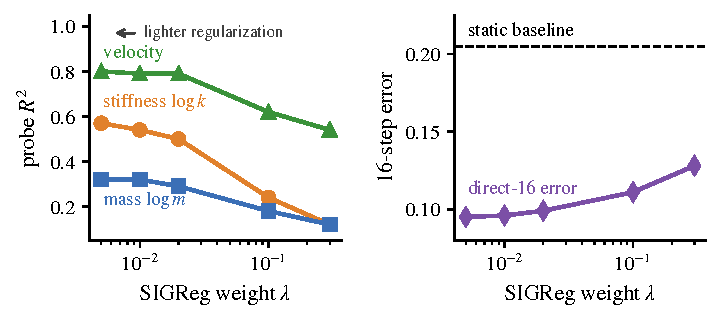
\includegraphics[width=0.72\linewidth]{fig_lambda.pdf}
\caption{\textbf{One knob, every readout.} Lightening the anti-collapse
weight $\lambda$ monotonically sharpens every physical probe (left) and
halves long-horizon prediction error against the static baseline (right);
training is stable across the full $60\times$ range. Arrow: direction of
lighter regularization.}
\label{fig:lambda}
\end{figure}

\begin{table}[H]
\caption{\textbf{The regularizer sweep behind Fig.~\ref{fig:lambda}.} VFX, contact-window probes; 16-step direct error in arena units against a static baseline of $0.205$. Every readout sharpens monotonically as $\lambda$ lightens.}
\label{tab:lambda}
\begin{center}
\small
\begin{tabular}{lccccc}
\toprule
\rowcolor{tabhead} $\lambda$ & $0.3$ & $0.1$ & $0.02$ & $0.01$ & $0.005$ \\
\midrule
$\log k$ & $0.12$ & $0.24$ & $0.50$ & $0.54$ & $0.57$ \\
$\log m$ & $0.12$ & $0.18$ & $0.29$ & $0.32$ & $0.32$ \\
velocity & $0.54$ & $0.62$ & $0.79$ & $0.79$ & $0.80$ \\
direct-16 error & $0.128$ & $0.111$ & $0.099$ & $0.096$ & $0.095$ \\
\bottomrule
\end{tabular}
\end{center}
\end{table}

Finally, the data-coverage intervention of \S\ref{sec:threefactors}: the
identical VFX objective trained on 95\%-glide data and evaluated on the
standard probe distribution falls to $\log k$ $0.05$, $\log m$ $0.11$,
position $0.87$, velocity $0.58$, against $0.50/0.29/0.98/0.79$ with
standard coverage---acquisition runs on the gradient mass the data supplies.

\subsection{The attribute matrix and its dose--responses}
\label{app:matrix}

The matrix asks which \emph{attributes} of a physical parameter decide
whether a prediction-trained latent acquires it. Each cell pairs a parameter
with its recoverability certificate (the appropriate instrument per cell:
GRU sequence probes for ratio-type parameters, linear and GRU probes for the
linear cells, the physics-informed estimator for drag) and scores
acquisition as model readout over certificate---a comparison to the best
simple estimator, since certificates are lower bounds.

\begin{table}[H]
\caption{\textbf{The attribute matrix in full.} Each cell pairs a parameter with its certificates and scores acquisition as model readout over certificate. The fast parameter is acquired beyond its linear trace; slow parameters only up to it.}
\label{tab:matrixfull}
\begin{center}
\small
\begin{tabular}{llcccc}
\toprule
\rowcolor{tabhead} Cell & Parameter & Linear cert.\ & Recurrent cert.\ & Model & vs.\ recurrent \\
\midrule
fast$\times$ratio & stiffness $k$ & ${\approx}0$ & $0.87$ & $0.50$--$0.62$ & $0.6$--$0.7$ \\
slow$\times$linear, $b \in \pm 0.5$ & force bias & $0.13$ & $0.92$ & $0.13$ & $0.14$ \\
slow$\times$linear, $b \in \pm 1.5$ & force bias & $0.51$ & $0.96$ & $0.39$ & $0.41$ \\
slow$\times$linear, $b \in \pm 2.5$ & force bias & $0.65$ & $0.96$ & $0.65$ & $0.68$ \\
slow$\times$ratio, gated & drag $\gamma$ & ${\approx}0$ & $0.89$ & $0.13$ & $0.15$ \\
slow$\times$ratio, ungated & actuation gain $g$ & $-0.01$ & $0.69$ & $-0.01$ & $\mathbf{0.0}$ \\
\bottomrule
\end{tabular}
\end{center}
\end{table}

Down the bias family the model tracks its \emph{linear} certificate and
never its recurrent one, which stays near $0.95$ at every signal level; the
fast parameter alone is acquired beyond its linear trace. The two
dose--responses below rule out variance-share as the missing explanation.

\textbf{The coordinate test.} Supplying a log-speed input channel (computed
from the frozen flow sensor) linearizes glide decay. The linear $\gamma$
certificate under this coordinate---ridge regression on log-speed sequences
over glide windows ($696/351$ fit/test)---is $0.52$, and the trained model's
glide-window readout rises from $0.08$ to $0.33$ (ridge; the MLP probe is
unstable on this small subset), with stiffness, mass, and velocity
unchanged. The functional glide test does not improve ($0.114$ against a
median-$\gamma$ reference of $0.054$): the linear trace is acquired; its
exponentiation into position forecasts is not.

\textbf{Pixel-derived certificates.} Replacing simulator object state with
pixel-centroid estimates (finger disk masked using proprioception, 3-frame
smoothing): the recurrent certificate reads $m/\gamma/k = 0.72/0.43/0.78$
(state-based $0.86/0.70/0.87$), and a centroid-based analytic $\gamma$
estimator degrades to $0.05$---sub-pixel velocity precision is the binding
constraint. Model readouts against pixel certificates: stiffness
$0.64$--$0.79$, mass $0.43$, drag $0.30$.

\textbf{Constructing the cells.} The slow$\times$linear cell required
four constructions; the certificate gate rejected the first three, each
instructively: (i)~a per-episode drift acceleration is unrecoverable from
16-step windows because it enters $\dot v = a_d - \gamma v$ jointly with
per-episode drag (certificate $0.03$); (ii)~fixing $\gamma$ still fails a
\emph{linear} certificate because the drift is readable only on contact-free
frames---temporal gating again; (iii)~a multiplicative actuation gain is
inherently ratio-type ($g = \Delta v / (F a)$; certificate $-0.00$). The
accepted construction is an additive per-episode force bias on the agent:
$\Delta v = (Fa + b - cv)\,\mathrm{d}t$ is linear in $(a, v, b)$, ungated, and
sub-pixel per step. Its linear certificate is $0.13$; the recurrent
certificate ($0.92$) later exposed how loose that bound is, which is what
motivated the two-certificate protocol and the three-level sweep in the
table. The rejected actuation gain then
serves as the slow$\times$ratio$\times$ungated cell in its own right:
regenerated as a dedicated corpus ($g \in [0.85, 1.15]$ multiplying the
commanded force), its linear certificate fails as designed ($-0.013$) while a
GRU sequence certificate recovers it at $0.689$; the trained model's trunk
reads it at $-0.011$ (ridge) / $-0.010$ (MLP)---none of its recurrent
certificate---in
a run whose stiffness, mass, and position probes are at normal levels
($0.34$/$0.20$/$0.96$).

\textbf{Dose--response 1: reweighting toward the blind parameter.} Sampling
zero-contact (glide) episodes at relative weights $\{1,4,16,64\}$
reallocates the expected loss mass of glide segments from $32\%$ to $97\%$,
with data, probe sets, and certificates unchanged. Linear decodability of
$\gamma$ creeps upward but never approaches its certificate ($0.89$); the
functional glide test \emph{worsens}; and the acquired parameters pay the
price.

\begin{table}[H]
\caption{\textbf{Reweighting toward the blind parameter.} As the glide loss share rises, $\gamma$'s decodability creeps upward, its functional test \emph{worsens}, and the acquired parameters degrade.}
\label{tab:dose1}
\begin{center}
\small
\begin{tabular}{lcccc}
\toprule
\rowcolor{tabhead} glide loss share & $32\%$ & $65\%$ & $88\%$ & $97\%$ \\
\midrule
$\gamma$ (glide windows) & $0.08$ & $0.15$ & $0.21$ & $0.27$ \\
functional glide error (median-$\gamma$ ref.\ $0.054$) & $0.098$ & $0.108$ & $0.116$ & $0.136$ \\
$\log k$ & $0.42$ & $0.34$ & $0.20$ & $0.10$ \\
velocity & $0.85$ & $0.79$ & $0.70$ & $0.65$ \\
\bottomrule
\end{tabular}
\end{center}
\end{table}

\textbf{Dose--response 2: starving an acquired parameter.} Scaling the
contact-frame touch-loss weight down from its default drives stiffness to
exactly zero, parameter-specifically---mass dips mildly and $\gamma$ does
not move---again with data and certificates unchanged.

\begin{table}[H]
\caption{\textbf{Starving an acquired parameter.} Scaling the contact-frame touch-loss weight down drives stiffness to zero parameter-specifically, with data and certificates unchanged.}
\label{tab:dose2}
\begin{center}
\small
\begin{tabular}{lcccc}
\toprule
\rowcolor{tabhead} contact-frame touch weight & $4$ (default) & $1$ & $0.25$ & $0$ \\
\midrule
$\log k$ & $0.50$ & $0.37$ & $0.12$ & $-0.005$ \\
$\log m$ & $0.29$ & $0.28$ & $0.26$ & $0.21$ \\
$\gamma$ & $0.12$ & $0.14$ & $0.13$ & $0.14$ \\
\bottomrule
\end{tabular}
\end{center}
\end{table}

Together: loss share is a continuous throttle on parameters the objective
can acquire, and no amount of it unblinds the slow$\times$ratio conjunction.

\begin{figure}[t]
\centering
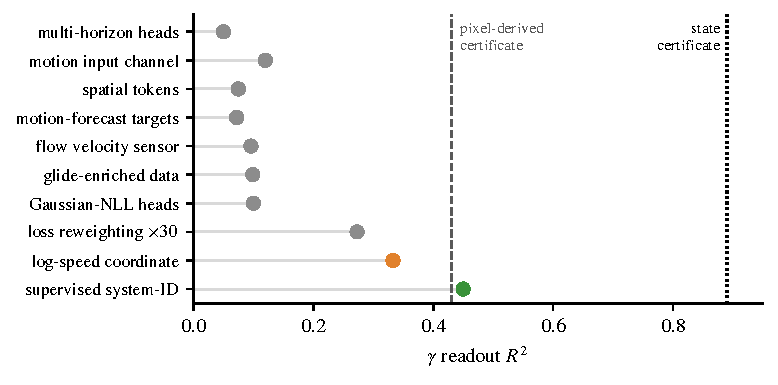
\includegraphics[width=0.62\linewidth]{fig_gamma_ledger.pdf}
\caption{\textbf{The $\gamma$ intervention ledger.} Best $\gamma$ readout
under every intervention deployed against drag, against the pixel-derived
(dashed) and state-trajectory (dotted) certificates. Prediction-side
mechanisms (gray) plateau; only a linearizing sensed coordinate (orange) and
direct supervision (green) move it.}
\label{fig:ledger}
\end{figure}

\textbf{The $\gamma$ intervention ledger} (Fig.~\ref{fig:ledger}). For
completeness, every prediction-side mechanism deployed against drag, with
its outcome:
multi-horizon heads ($\gamma$: $0.00 \rightarrow 0.05$), a motion input
channel ($\rightarrow 0.12$ plateau), spatial tokens (no gain),
magnitude-weighted motion-forecast targets (no gain), a frozen flow velocity
sensor (velocity readout $0.79 \rightarrow 0.88$; the $\gamma$ plateau
unchanged), and glide-enriched data (no gain). The functional test evaluates
the model's own direct 16-step predictions on certified pure-glide windows
against analytic references: an estimator that knows the true $\gamma$ errs
by $0.0002$, one that assumes the population-median $\gamma$ by $0.049$, a
static predictor by $0.144$; the model sits above the median-$\gamma$
reference at every loss share (Dose--response~1). $\gamma$-specific
information is absent \emph{functionally}, not merely linearly.

\subsection{Objective-attribution controls}
\label{app:controls}

Both controls keep the VFX trunk, data, probes, and optimizer, and change
only the objective. The supervised system-identification head shows the
substrate carries every parameter the moment the objective asks for it; the
reconstruction objective shows the blind region is not specific to latent
targets, while the touch-target mechanism transfers.

\begin{table}[H]
\caption{\textbf{Objective-attribution controls.} Same trunk, data, probes, and optimizer; only the objective changes. Ridge readouts with early-stopped MLP in parentheses.}
\label{tab:controls}
\begin{center}
\small
\begin{tabular}{lcccccc}
\toprule
\rowcolor{tabhead} & \multicolumn{3}{c}{ridge (MLP), contact windows} & & & \\
\cmidrule(lr){2-4}
\rowcolor{tabhead} Objective & $\log m$ & $\gamma$ & $\log k$ & position & velocity & direct-16 \\
\midrule
\rowcolor{tabours} VFX, latent targets & $0.29$ ($0.26$) & $0.12$ ($0.06$) & $0.50$ ($0.50$) & $0.98$ & $0.79$ & $0.098$ \\
\;\;+ system-ID head & $0.72$ ($0.70$) & $0.45$ ($0.39$) & $0.91$ ($0.91$) & $0.98$ & $0.78$ & $0.101$ \\
VFX, Gaussian-NLL & $0.31$ ($0.29$) & $0.10$ ($0.07$) & $0.49$ ($0.48$) & $1.00$ & $0.88$ & $0.143$ \\
V, reconstruction & $0.16$ ($0.00$) & $0.08$ ($0.00$) & $-0.01$ ($-0.10$) & $0.75$ & $0.47$ & --- \\
VFX, reconstruction & $0.19$ ($0.19$) & $0.03$ ($-0.04$) & $0.61$ ($0.63$) & $0.95$ & $0.64$ & --- \\
\bottomrule
\end{tabular}
\end{center}
\end{table}

The reconstruction rows have no direct-16 entry because their latent
prediction heads receive no gradient (App.~\ref{app:training}); the probes
are the comparable quantity. The Gaussian-NLL row is the minimal
belief-adjacent variant: heteroscedastic variance heads reweight gradients
(velocity and position readouts improve) but leave the conditional-mean
optimum---and the blind region---unchanged.

\textbf{Composition probes.} At the multi-horizon operating point, finger,
object, and relative object--finger position probes saturate for every
variant ($0.96$--$1.00$): the composition effect of \S\ref{sec:pressure}
belongs to the single-horizon regime of Table~\ref{tab:targets}, where
multi-horizon pressure is absent and object position differentiates
($0.09/0.17/0.58$).

\subsection{Closed-loop planning}
\label{app:planning}

Push-to-goal with the same planner, budget, and environment for every
representation (\S\ref{sec:planning}): CEM over smooth two-knot action
programs, scored by the direct $\Delta{=}4/16$ heads, replanning every 4
steps; Fig.~\ref{fig:plan} contrasts two representations on one held-out
episode. Deployment
follows the map: smooth action candidates (forward heads respond
faithfully where trained) and direct-$\Delta$ scoring, not composed
rollouts (\S\ref{sec:lazy}).

\begin{table}[H]
\caption{\textbf{Closed-loop planning.} Push-to-goal with an identical planner, budget, and environment for every representation: control tracks the state content of the latent.}
\label{tab:planning}
\begin{center}
\small
\begin{tabular}{lcccc>{\columncolor{tabours}}c}
\toprule
\rowcolor{tabhead} Controller & random & V & VX$_t$ & VX$_p$ & VFX \\
\midrule
goal-region reach & $1\%$ & $20\%$ & $38\%$ & $44\%$ & \best{$57\%$} \\
median distance improvement & $0.00$ & $0.02$ & $0.15$ & $0.18$ & \best{$0.24$} \\
\bottomrule
\end{tabular}
\end{center}
\end{table}

\begin{figure}[t]
\centering
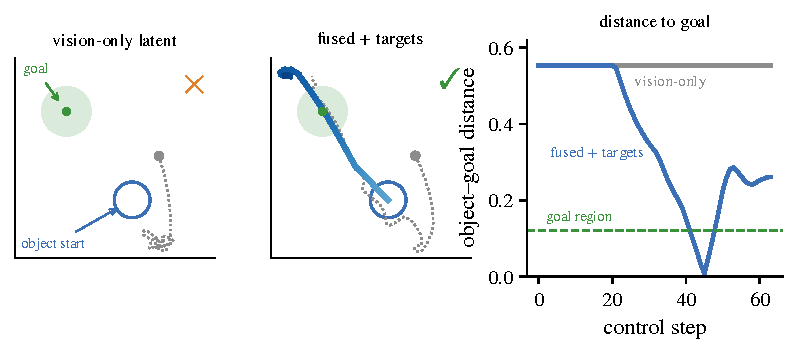
\includegraphics[width=0.94\linewidth]{fig_plan.pdf}
\caption{\textbf{The same task on two frozen latents.} One held-out
episode, one planner, one budget; only the representation differs. Object
path colored by time, finger path dotted, hollow circle the object's start,
shaded disc the goal region. Left: the object-blind vision-only latent
($\times$) --- the planner never reaches the object, and the distance never
moves off its initial $0.55$. Center: the full model ($\checkmark$)
maneuvers the finger to the push side, then drives the object through the
goal region. Right: both episodes as object--goal distance.}
\label{fig:plan}
\end{figure}

\subsection{Real-robot results in full}
\label{app:real}

Three protocol notes apply throughout. Sensor streams are per-column clipped
to robust ranges ($0.1$--$99.9$ percentiles) before whitening. Contact-onset
labels mark $\|F\| > 10$\,N within the next 4 steps; onset base rates differ
across configurations ($2.75\%$ on cfg7, $0.64\%$ on cfg1), so AUC values
compare within, not across, configurations. Every IID/OOD pair is a
probe-episode / held-out-task split.

\textbf{The pilot configuration (KUKA, cfg7).} Far camera;
$896$ episodes, $56$ tasks, static baseline $3.8$\,cm.

\begin{table}[H]
\caption{\textbf{KUKA (cfg7): all four variants.} Readouts, 16-step prediction, and contact anticipation on the pilot configuration.}
\label{tab:kuka}
\begin{center}
\small
\begin{tabular}{lcccc}
\toprule
\rowcolor{tabhead} & force (IID/OOD) & position (IID/OOD) & 16-step (cm) & AUC (IID/OOD) \\
\midrule
V & $-0.05$ / $-0.49$ & $0.76$ / $0.48$ & $8.2$ & $0.70$ / $0.54$ \\
VX & $-0.02$ / $-0.70$ & $0.75$ / $0.50$ & $5.8$ & $0.77$ / $0.69$ \\
VX$_t$ & $-0.04$ / $-0.61$ & $0.77$ / $0.46$ & $6.2$ & $0.80$ / $0.72$ \\
\rowcolor{tabours} VFX & $0.87$ / $0.56$ & $0.98$ / $0.98$ & $1.5$ & $0.86$ / $0.70$ \\
\bottomrule
\end{tabular}
\end{center}
\end{table}

\textbf{Viewpoint study (cfg7).} Rows report the camera-only quantities at
each viewpoint: force from VX, position from the best camera-only variant
at that viewpoint. VFX is stable across all three ($0.98$ position,
$0.84$--$0.90$ force).

\begin{table}[H]
\caption{\textbf{Viewpoint selects observables (cfg7).} A far view carries pose, a close-up carries contact cues, and two views take their union.}
\label{tab:viewpoint}
\begin{center}
\small
\begin{tabular}{lccc}
\toprule
\rowcolor{tabhead} camera & camera-only force & camera-only position (IID/OOD) & 16-step (cm) \\
\midrule
far view & $-0.02$ & $0.76$ / $0.48$ & $5.8$ \\
close-up & $+0.10$ & $0.48$ / $0.17$ & --- \\
two views & $0.08$ & $0.81$ / $0.60$ & $5.0$ \\
\bottomrule
\end{tabular}
\end{center}
\end{table}

\textbf{Scaling within one embodiment (Flexiv, cfg1).} The numbers
behind Fig.~\ref{fig:scissors}; static baseline $3.3$\,cm. At full scale the
$+50\%$-compute control leaves V's position at $0.16$, and V's open-loop
16-step rollout is $15.7$\,cm.

\begin{table}[H]
\caption{\textbf{The four-arm factorial across scale (Flexiv, cfg1).} Every arm missing information or prediction pressure is flat in scale; only the full objective converts data into held-out gains.}
\label{tab:cfg1}
\begin{center}
\small
\begin{tabular}{llcccccc}
\toprule
\rowcolor{tabhead} arm & episodes & force IID & force OOD & pos.\ IID & pos.\ OOD & 16-step (cm) & AUC OOD \\
\midrule
V & 800 & $-0.07$ & $-0.32$ & $0.18$ & $-0.06$ & $11.7$ & $0.75$ \\
 & 2000 & $-0.05$ & $-0.35$ & $0.14$ & $0.04$ & $12.5$ & $0.70$ \\
 & 4258 & $-0.06$ & $-0.30$ & $0.23$ & $0.02$ & $12.0$ & $0.62$ \\
\midrule
VX & 800 & $-0.03$ & $-0.31$ & $0.33$ & $0.30$ & $10.0$ & $0.76$ \\
 & 2000 & $-0.03$ & $-0.26$ & $0.30$ & $0.22$ & $10.2$ & $0.73$ \\
 & 4258 & $-0.04$ & $-0.27$ & $0.34$ & $0.24$ & $10.4$ & $0.77$ \\
\midrule
VF & 800 & $0.15$ & $-0.16$ & $0.95$ & $0.95$ & $2.9$ & $0.78$ \\
 & 2000 & $0.15$ & $-0.19$ & $0.95$ & $0.96$ & $2.8$ & $0.74$ \\
 & 4258 & $0.15$ & $-0.06$ & $0.96$ & $0.96$ & $2.7$ & $0.85$ \\
\midrule
\rowcolor{tabours} VFX & 800 & $0.90$ & $0.86$ & $0.96$ & $0.96$ & $2.2$ & $0.88$ \\
\rowcolor{tabours}  & 2000 & $0.91$ & $0.85$ & $0.96$ & $0.97$ & $2.5$ & $0.88$ \\
\rowcolor{tabours}  & 4258 & $0.92$ & $0.89$ & $0.97$ & $0.97$ & $2.3$ & $0.89$ \\
\bottomrule
\end{tabular}
\end{center}
\end{table}

\textbf{Cross-robot differences are a viewpoint effect.} The apparent
V degradation across robots is the viewpoint effect of Table~\ref{tab:viewpoint}, not a scale effect.

\begin{table}[H]
\caption{\textbf{Cross-embodiment comparison.} The two-point contrast that motivated the within-embodiment scaling curves.}
\label{tab:crossemb}
\begin{center}
\small
\begin{tabular}{lcc>{\columncolor{tabours}}c>{\columncolor{tabours}}c}
\toprule
\rowcolor{tabhead} & \multicolumn{2}{c}{V (vision-only)} & \multicolumn{2}{c}{VFX (multimodal)} \\
\cmidrule(lr){2-3}\cmidrule(lr){4-5}
\rowcolor{tabhead} & cfg7 & cfg1 ($5\times$) & cfg7 & cfg1 ($5\times$) \\
\midrule
Position readout (IID) & $0.76$ & $0.23$ & $0.98$ & $0.97$ \\
Position readout (OOD) & $0.48$ & $0.02$ & $0.98$ & $0.97$ \\
Force readout (OOD) & --- & --- & $0.56$ & $0.89$ \\
Contact anticipation AUC (OOD) & $0.54$ & $0.62$ & $0.70$ & $0.89$ \\
16-step prediction (IID, cm) & $8.2$ & $15.7$ & $1.5$ & $2.2$ \\
\quad static baseline (cm) & $3.8$ & $3.3$ & $3.8$ & $3.3$ \\
\bottomrule
\end{tabular}
\end{center}
\end{table}

\textbf{Untrained-encoder bounds.} Random weights, identical probe
protocol: frame-level readout of fused inputs is passthrough, and
prediction is not. Figure~\ref{fig:forceread} plots the four arms'
current-force readout against this bound---the retention view of the
factorial whose learning view (forecasting) appears in
Fig.~\ref{fig:scissors}.

\begin{figure}[t]
\centering
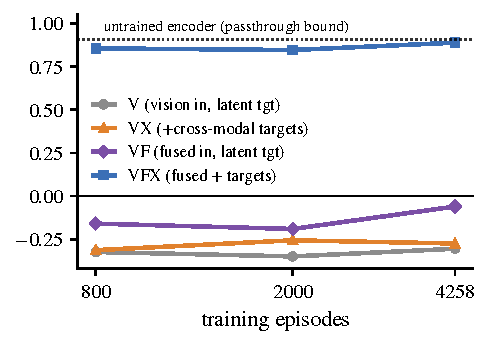
\includegraphics[width=0.5\linewidth]{fig_force_readout.pdf}
\caption{\textbf{Current-force readout is passthrough-bounded.} Held-out
force readout of the four arms against the untrained-encoder bound
(dotted): VX lacks the information, VF destroys it, VFX saturates the
bound---which is why the main figure reports force \emph{forecasting}
instead.}
\label{fig:forceread}
\end{figure}

\begin{table}[H]
\caption{\textbf{Untrained-encoder bounds.} Random weights, identical probe protocol: frame-level readout of fused inputs is passthrough, and prediction is not.}
\label{tab:rand}
\begin{center}
\small
\begin{tabular}{lcccc}
\toprule
\rowcolor{tabhead} architecture & force (IID/OOD) & position (IID/OOD) & 16-step & AUC (IID/OOD) \\
\midrule
VFX, untrained & $0.94$ / $0.91$ & $0.97$ / $0.98$ & $23$\,m & $0.87$ / $0.88$ \\
V, untrained & $-0.01$ / $-0.16$ & $0.21$ / $0.13$ & $185$\,m & $0.72$ / $0.51$ \\
\bottomrule
\end{tabular}
\end{center}
\end{table}

\textbf{Future-force forecasting.} R\textsuperscript{2} of predicted force
at $t{+}\Delta$ (IID/OOD) against a persistence baseline that repeats the
last observed force. Forecasting is the passthrough-immune force metric:
VFX doubles the persistence baseline at $0.4$\,s while camera-only VX
cannot match it.

\begin{table}[H]
\caption{\textbf{Future-force forecasting.} R\textsuperscript{2} of predicted force at $t{+}\Delta$ against a persistence baseline that repeats the last observed force---the passthrough-immune force metric.}
\label{tab:futforce}
\begin{center}
\small
\begin{tabular}{lcc}
\toprule
\rowcolor{tabhead} & $\Delta{=}1$ ($0.1$\,s) & $\Delta{=}4$ ($0.4$\,s) \\
\midrule
\rowcolor{tabours} VFX & \best{$0.72$ / $0.68$} & \best{$0.47$ / $0.51$} \\
VX & $0.18$ / $-0.07$ & $0.15$ / $-0.05$ \\
persistence & $0.65$ / $0.61$ & $0.24$ / $0.31$ \\
\bottomrule
\end{tabular}
\end{center}
\end{table}

Across the scaling arms, VFX's held-out $\Delta{=}4$ forecast rises
$0.39 \rightarrow 0.50 \rightarrow 0.51$ ($800/2{,}000/4{,}258$ episodes)
while VX sits at $-0.05/-0.11/-0.05$: the center panel of
Fig.~\ref{fig:scissors} in numbers. Paired episode-bootstrap $95\%$ CIs of
the model$-$persistence difference exclude zero at every scale for VFX
($[+0.01, +0.17]$ at $800$; $[+0.14, +0.28]$ at $4{,}258$) and are strictly
negative for VX ($[-0.55, -0.15]$), so neither the advantage nor its growth
with scale is a task-composition artifact.

\end{document}
